\documentclass{article}
\usepackage[UTF8, heading = false, scheme = plain]{ctex}

\usepackage{geometry}
\geometry{b5paper,left=2cm,right=2cm,top=2cm,bottom=2cm}

\usepackage{color}
\usepackage{amsfonts}
\usepackage{amsmath}

\linespread{1.5}

\usepackage[colorlinks,
            linkcolor=red,
            anchorcolor=blue,
            citecolor=green
            ]{hyperref}

\usepackage{listings}
\usepackage{fontspec}
\newfontfamily\monaco{Monaco}
\definecolor{dkgreen}{rgb}{0,0.6,0}
\definecolor{gray}{rgb}{0.5,0.5,0.5}
\definecolor{mauve}{rgb}{0.58,0,0.82}
\lstset{ %
  basicstyle=\footnotesize\monaco,       % the size of the fonts that are used for the code
  numbers=left,                   % where to put the line-numbers
  numberstyle=\footnotesize\monaco\color{gray},  % the style that is used for the line-numbers
  numbersep=5pt
  stepnumber=1,                   % the step between two line-numbers. If it's 1, each line
                                  % will be numbered
  numbersep=5pt,                  % how far the line-numbers are from the code
  backgroundcolor=\color{white},      % choose the background color. You must add \usepackage{color}
  showspaces=false,               % show spaces adding particular underscores
  showstringspaces=false,         % underline spaces within strings
  showtabs=false,                 % show tabs within strings adding particular underscores
  frame=single,                   % adds a frame around the code
  rulecolor=\color{black},        % if not set, the frame-color may be changed on line-breaks within not-black text (e.g. commens (green here))
  tabsize=4,                      % sets default tabsize to 2 spaces
  captionpos=t,                   % sets the caption-position to bottom
  breaklines=true,                % sets automatic line breaking
  breakatwhitespace=false,        % sets if automatic breaks should only happen at whitespace
  title=\lstname,                   % show the filename of files included with \lstinputlisting;
                                  % also try caption instead of title
  keywordstyle=\color{blue},          % keyword style
  commentstyle=\color{dkgreen},       % comment style
  stringstyle=\color{mauve},         % string literal style
  escapeinside={\%*}{*)},            % if you want to add LaTeX within your code
  morekeywords={*,...}               % if you want to add more keywords to the set
}

\usepackage{amssymb} 

\setlength{\parindent}{2em}

\renewcommand{\G}{\mathbb{G}}
\newcommand{\Z}{\mathbb{Z}}
\newcommand{\Q}{\mathbb{Q}}
\newcommand{\F}{\mathbb{F}}

\newcommand{\Sbox}{\textsf{Sbox}}
\newcommand{\code}[1]{\lstinline!#1!}

%%%%%%%处理下划线:_%%%%%%%%%
\usepackage{underscore}
%%%%%%%处理下划线:_%%%%%%%%%

\setlength{\parindent}{2.1em}

\begin{document}

\title{深入理解Bitcoin钱包机制}
\author{Jia, longcpp \\ \small{yin.jia987@gmail.com, longcpp9@gmail.com}}

\maketitle


在比特币系统中,私钥代表着对比特币的完全控制,用户在发送交易时需要直接与私钥打交道。
但由于私钥本身是一串256比特的二进制串,直接以二进制形式访问私钥对用户来说非常不友好。
为了方便用户记录和识别,私钥衍生出了Hex,WIF,WIF-compressed等不同形式,
它们与256bit二进制串相比长度更短,易于辨别。但由于一个地址就对应了一对公私钥,
这些零散的公私钥管理起来十分不便,给用户使用带来了困难。

为了更好地对于私钥进行保护和管理,以及优化用户体验,BIP中一些协议对此进行了探索:
BIP32提出了分层确定性钱包的概念,允许用户从一个seed确定性地派生出一棵密钥树,
方便在不同钱包客户端之间进行切换,并使得公私钥的派生过程可以独立进行。
BIP39则给出了seed的生成方法,并且允许将该seed与一组助记词对应起来,方便用户理解和记忆。
BIP38针对私钥的安全性,提出了对私钥进行加密保护的方法,与之前相比,
用户只需要多记忆一个passphrase,同时获得了更高的安全性。

上述的BIP协议主要是在如何简化用户与钱包软件的交互、以及在不过多增加用户负担的情况下提高安全性等方面进行的探索,
主要是希望由用户掌握一个较短的、方便记忆的字符串,通过密码学的方法,派生出不同用途的密钥(签名、加密)。
因此这些方案中除了基本的加密(AES),签名(ECDSA)算法之外,用到的另外一类算法就是Password-based Key Derivation Function(PBKDF)。
下面首先会对涉及到的PBKDF做简要介绍,然后逐一说明每个BIP的原理、功能。

\section{Password-based Key Derivation Function}
PBKDF用来从一个较短的便于记忆的password派生出密码学方案中使用的密钥,通常在password之外还有一些其他参数如salt、
iteration count等。这类函数通常是computationally intensive,即需要的计算量较大。
对于合法用户,每次操作只需进行一次派生计算,因此计算量是可以忽略的。
而对暴力攻击,攻击者可能需要执行上亿次计算,因此它大幅增加了攻击者的计算难度。
并且此类算法支持随着计算机硬件的发展做对计算难度进行灵活的调整,使用起来十分方便。

\subsection{PBKDF2}
PBKDF2全称为Password-Based Key Derivation Function 2,在PKCS\#5
中取代了输出长度不大于160bit的PBKDF1作为该规范推荐的密钥派生函数。
BIP39协议使用该函数从助记词组派生一个随机串,该随机串用作BIP32 HD(Hierarchical Deterministic)
钱包中生成主密钥对的seed。  PBKDF2最早被包含在PKCS\#5中发表,后来该规范又被IETF以RFC 
2898\footnote{https://tools.ietf.org/html/rfc2898}重新发表。在2017年发布的RFC8018中,仍然建议用它来做password hashing。

在PBKDF中,由于用户的passphrase取值空间一般较小,攻击者在进行暴力攻击时比较容易。
Salt作为一段均匀随机分布的比特串,不需要保密,目的是为了增加攻击者的搜索空间。
同时当salt足够长时(如64bit),攻击者无法通过预计算存储相应的计算结果,从而降低了攻击的可行性。

\subsection{Scrypt算法}
Scrypt算法由Colin Percival设计,与PBKDF2相比,该算法在执行时对内存的消耗较高,
限制了利用硬件并行实现来划分搜索空间从而降低暴力攻击复杂度的可行性,
以此来抵抗大规模的专用硬件攻击(即使用ASIC来加速暴力攻击的计算过程)。
BIP38协议使用Scrypt算法作为密钥派生函数,从passphrase派生AES的加密密钥。 
 
Scrypt算法定义如\ref{Scrypt},用户可以根据当前CPU、内存的发展情况、以及要求的并行度对
N,r,p参数进行调节,从而调整算法对CPU/内存的消耗。

其中,scryptROMix\ref{scryptROMix}算法用来产生一个expensive-cost 的salt,Scrypt算法对内存的消耗即来源于它。在执行时,它会产生一组长度为N的伪随机比特串(如下,$V[i]$),
同时以一种伪随机的顺序对该比特串进行访问,这就导致攻击者必须有足够的内存来存储它。
并且该比特串的计算是比较费时的,因此攻击者经过对时间和空间进行权衡的结果,
要么是对内存资源要求不高但运行很慢,要么是效率较高但内存消耗较大。

\begin{algorithm}[tbp]\footnotesize
\caption{PBKDF2}
\label{PBKDF2}
  	\begin{algorithmic}[1]
	    \REQUIRE ~~\\ 
	    PRF: pseudorandom function of two parameters with output length hLen (Optional)\\
	    Password: the master password from which a derived key is generated\\
	    Salt: a sequence of bits, known as a cryptographic salt\\
	    c: the number of iterations desired\\
	    dkLen: the desired bit-length of the derived key\\
	    \ENSURE ~~\\
	    DK: the generated derived key\\
	    \STATE If $dkLen > (2^{32} - 1) * hLen$, output "derived key too long" and stop;
	    \STATE Let $l$ be the number of $hLen$-octet blocks in the derived key,
	     rounding up, and let $r$ the number of octets in the last block:  
			$$l =\lceil (dklen/hlen) \rceil $$ 
			$$r =dklen -(l-1)*hlen;$$		
		\STATE For each block of the derived key, apply the function $F$ defined 
		below to the password $P$, the salt $S$, 
	  	the iteration count $c$, and the block index to compute the block:
			$$T_1=F(P,S,c,1)$$
			$$T_2=F(P,S,c,2)$$
			$$\cdots$$
			$$T_l=F(P,S,c,l)$$ 
		where $F$ is defined as: $F(P,S,c,i)=U_1 \oplus U_2  \cdots \oplus U_c$ and
			$$U_1=PRF(P,S||INT(i))$$ 
			$$U_2=PRF(P,U_1)$$
			$$\cdots$$
			$$U_c=PRF(P,U_{c-1})$$
		Here, $INT (i)$ is a four-octet encoding of the integer i, most significant octet first.
		\STATE Concatenate the blocks and extract the first $dkLen$ octets to 
		produce a derived key $DK$:  
			$$DK=T_1||T_2||\cdots|| T_l<0,\cdots r-1>$$
		\RETURN the derived key $DK$.		
    \end{algorithmic}
\end{algorithm}
 

\begin{algorithm}[tbp]\footnotesize
\caption{Scrypt}
\label{Scrypt}
  	\begin{algorithmic}[1]
	    \REQUIRE ~~\\ 
	    Passphrase, the password string.\\
		Salt, a sequence of bits, known as a cryptographic salt.\\
		N, CPU/Memory cost parameter, must be larger than 1, a power of 2,
		 and less than $2^{(128 * r / 8)}$.\\
		r, Block size parameter.\\
		p, Parallelization parameter, a positive integer less than or equal 
		to $((2^{32}-1) * hLen) / MFLen$ where $hLen$ is 32 and $MFlen$ is $128 * r$.\\
		$dklen$, Intended output length in octets of the derived key; 
		a positive integer less than or equal to $(2^{32} - 1) * hLen$ where $hLen$ is 32.\\
	    \ENSURE ~~\\
	    DK: the generated derived key\\
	    \STATE Initialize an array $B$ consisting of $p$ blocks of $128 * r$ octets each:\\
			$B[0]||B[1]||\cdots B[p-1]=PBKDF2-HMAC-SHA256(P,S,1,p*128*r)$
		\FOR{$i=0$ to $p-1$} 
			\STATE $B[i]= scryptROMix(r,B[i],N)$   
		\ENDFOR 
		\STATE $DK=PBKDF2-HMAC-SHA256(P,B[0]||B[1]||\cdots B[p-1],1,dklen)$
		\RETURN the derived key $DK$.		
    \end{algorithmic}
\end{algorithm}
 
\begin{algorithm}[tbp]\footnotesize
\caption{scryptROMix}
\label{scryptROMix}
  	\begin{algorithmic}[1]
	    \REQUIRE ~~\\ 
	    r, Block size parameter.\\
		B, Input octet vector of length $128 * r$ octets.\\
		N, CPU/Memory cost parameter, must be larger than 1,
		 a power of 2, and less than $2^{(128 * r / 8)}$.\\
		Integerify($B[0]||B[1]||\cdots B[2*r-1]$ ), 
		the result of intepreting $B[2*r-1]$ as a little-endian integer.\\
	    \ENSURE ~~\\
	    B', Output octet vector of length $128 * r$ octets.\\
	    \STATE $X = B$
		\FOR{$i = 0$ to $N - 1$}  
			\STATE $V[i]=X$  
			\STATE $X=scryptBlockMix(X)$  
 		\ENDFOR 
		\FOR{$i=0 to N-1$}  
			\STATE $j=Integerify(X)$ mod $N$  
			\STATE $T=X \oplus V[j]$  
			\STATE $X=scryptBlockMix(T)$  
		\ENDFOR
		\RETURN $B'=X$	
    \end{algorithmic}
\end{algorithm}


\begin{algorithm}[tbp]\footnotesize
\caption{scryptBlockMix}
  	\begin{algorithmic}[1]
	    \REQUIRE ~~\\ 
	     r, Block size parameter\\
 		$B[0]||B[1]||\cdots B[2*r-1]$, input octet string (of size $128 * r$ octets), 
 		treated as $2 * r 64$-octet blocks, where each element in $B$ is a 64-octet block.\\
 		Salsa refers to Salsa20/8, which is reduced round function of Salsa20 Core.\\
	    \ENSURE ~~\\
	    $B'[0]||B'[1]||\cdots B'[2*r-1]$, output octet string.\\
	    \STATE $X = B[2*r-1]$
		\FOR {$i = 0$ to $2*r - 1$} 
			\STATE $T=X \oplus B[i]$  
			\STATE $X=Salsa(T)$  
			\STATE $Y[i]=X$
		\ENDFOR 
		\RETURN $B'=(Y[0],Y[2],\cdots,Y[2*r-2],Y[1],Y[3],\cdots, Y[2*r-1])$
    \end{algorithmic}
\end{algorithm}

\begin{lstlisting}[language = c, caption = Salsa20/8, label=lst-salsa20core]
#define R(a,b) (((a) << (b)) | ((a) >> (32 - (b)))) 
void salsa20_word_specification(uint32 out[16],uint32 in[16]) 
{

	int i; 
	uint32 x[16]; 
	for (i = 0;i < 16;++i) x[i] = in[i]; 
	for (i = 8;i > 0;i -= 2) { 
		x[ 4] ^= R(x[ 0]+x[12], 7); x[ 8] ^= R(x[ 4]+x[ 0], 9);
		x[12] ^= R(x[ 8]+x[ 4],13); x[ 0] ^= R(x[12]+x[ 8],18); 
		x[ 9] ^= R(x[ 5]+x[ 1], 7); x[13] ^= R(x[ 9]+x[ 5], 9); 
		x[ 1] ^= R(x[13]+x[ 9],13); x[ 5] ^= R(x[ 1]+x[13],18); 
		x[14] ^= R(x[10]+x[ 6], 7); x[ 2] ^= R(x[14]+x[10], 9); 
		x[ 6] ^= R(x[ 2]+x[14],13); x[10] ^= R(x[ 6]+x[ 2],18); 
		x[ 3] ^= R(x[15]+x[11], 7); x[ 7] ^= R(x[ 3]+x[15], 9); 
		x[11] ^= R(x[ 7]+x[ 3],13); x[15] ^= R(x[11]+x[ 7],18); 
		x[ 1] ^= R(x[ 0]+x[ 3], 7); x[ 2] ^= R(x[ 1]+x[ 0], 9); 
		x[ 3] ^= R(x[ 2]+x[ 1],13); x[ 0] ^= R(x[ 3]+x[ 2],18); 
		x[ 6] ^= R(x[ 5]+x[ 4], 7); x[ 7] ^= R(x[ 6]+x[ 5], 9); 
		x[ 4] ^= R(x[ 7]+x[ 6],13); x[ 5] ^= R(x[ 4]+x[ 7],18); 
		x[11] ^= R(x[10]+x[ 9], 7); x[ 8] ^= R(x[11]+x[10], 9); 
		x[ 9] ^= R(x[ 8]+x[11],13); x[10] ^= R(x[ 9]+x[ 8],18); 
		x[12] ^= R(x[15]+x[14], 7); x[13] ^= R(x[12]+x[15], 9); 
		x[14] ^= R(x[13]+x[12],13); x[15] ^= R(x[14]+x[13],18);

	}
 	for (i = 0;i < 16;++i) out[i] = x[i] + in[i];

}
\end{lstlisting}



\section{分层确定性钱包 (BIP32, BIP44)}

在遵循中本聪的每次交易都使用新地址的建议时,为了防止每次交易后都需要对新生成的公私钥进行备份,
钱包客户端需要维护一个预留的密钥池. 这种方式给用户在不同客户端之间进行切换, 以及钱包对用户私钥的管理带来了困难:
在切换时,用户需要导出导入所有相关地址的私钥,并且不能在不同的系统上同时使用钱包.
分层确定性钱包从根节点确定性派生密钥树的方法很好地解决了这个问题.

分层确定性钱包是由Pieter Wuille在2012年于BIP32中提出的.
分层确定性钱包中, 从根节点出发按照层级结构以一种确定性的方式从parent key 派生 child key,
从而建立起一棵由根节点完全派生的树.因此,当用户在两个支持该协议的不同客户端之间进行切换时,密钥的导入、
导出只需要复制根节点(主密钥)的信息,钱包可以根据根节点和该协议规定的派生方法确定性地派生出整棵密钥树.
因此,用户可以方便地在不同客户端之间切换,钱包也可以依据密钥的派生层级对密钥进行逻辑上的分层管理.
  
此外,该协议允许子私钥和子公钥的派生过程相互独立,
即父私钥可以派生出子私钥和子公钥,而父公钥只能派生出子公钥.
这种机制允许在不安全的环境中,在没有父私钥访问权限的情况下,
依然可以进行子公钥的派生,从而防止父私钥的泄露.
同时,钱包的树状结构有助于用户对访问权限进行选择性的共享
(这取决于共享的密钥所处的层级,以及共享的是私钥还是公钥).  

BIP32着重讲述分层确定性钱包的原理,对于客户端如何实现并没有做严格的限制,
因此,2014年,Marek Palatinus和Pavol Rusnak 
提出了BIP44, 旨在BIP32的基础上对钱包具体的实现方式,不同层级的逻辑含义进行了规定.

\subsection{BIP32: 分层确定性钱包的密钥派生}

在使用该协议从父节点派生子节点时,实际上使用的是512比特的扩展密钥$(k,c)/(K,c)$,
其中$k$代表私钥, $K$代表公钥, $c$则称为链码(Chain Code),作为额外的256比特的熵.
对于扩展公私钥对,其中只有公私钥部分不同,链码是相同的.
 
每一个扩展密钥至多可以有$2^{31}$个平凡子密钥(Normal Child Key)和$2^{31}$个增强子密钥(Hardened Child Key), 
平凡子密钥对应的索引(Index)从0到$2^{31}-1$, 增强子密钥的索引则从$2^{31}$ 到$2^{32}-1$.
为便于表示, 我们用$i_H$表示增强子密钥的索引 $i+2^{31}$. 增强子密钥的引入是为了增强整个方案的安全性,
具体原理在Section~\ref{sec-security}~一节会详细介绍. 
下面首先介绍从父私钥(Private Parent Key)到子私钥(Private Child Key)的派生过程.

%\subsubsection{父私钥派生子私钥}
 
%\begin{figure}[h]
%\centering
%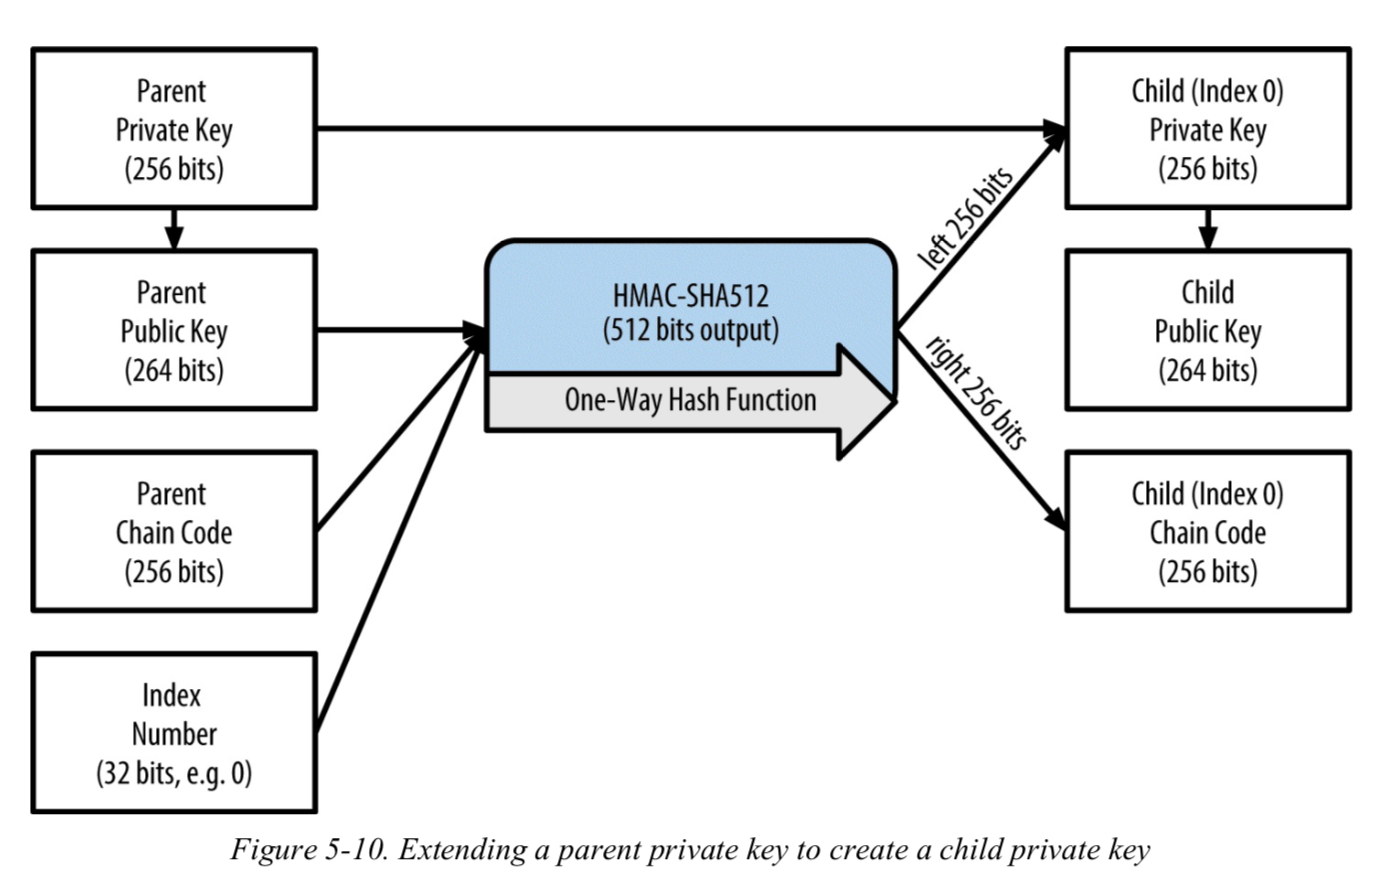
\includegraphics[width=.7\textwidth]{./CKDpriv.png}
%\caption{Normal child 的派生过程(图片来自《Master Bitcoin》)}\label{fig-parsesig}
%\end{figure}
 
\begin{algorithm}[h]\footnotesize
\caption{子私钥派生算法}\label{algo-drc-priv}
  	\begin{algorithmic}[1]
	    \STATE 函数 $\textsf{CKDpriv}((k_{par}, c_{par}), i) \rightarrow (k_i, c_i)$ 从父扩展私钥计算子扩展私钥:
		\STATE 判断索引$i$是否大于等于$2^{31}$, 也即判断子密钥的类型
		\IF {hardened child}
			\STATE let $I = \textsf{HMAC-SHA512}(Key = c_{par}, Data = 0x00 || ser_{256}(k_{par}) || ser_{32}(i))$
		\ELSE
			\STATE let $I = \textsf{HMAC-SHA512}(Key = c_{par}, Data = ser_P(k_{par}G) || ser_{32}(i))$
		\ENDIF
		\STATE 拆分$I$为两个32字节: $I_L || I_R = I, I_L = I[0,\cdots,31], I_R = I[32, \cdots, 63]$.
		\STATE 子私钥 $k_i = parse_{256}(I_L) + k_{par} \mod n $, 对应的链码$c_i = I_R$.
		\STATE 如果$parse256(I_L) \geq n$或者$k_i = 0$, 则计算结果不合法,此时递增$i$并重新计算.
    \end{algorithmic}
\end{algorithm}

在上述算法的第4步中, $Data$参数中的前缀$0x00$字节将私钥补齐为33个字节,与压缩形式的公钥(第6步)一样长.
而第10步中,计算结果不合法发生的概率大概为$1/2^{127}$.
根据上述算法也可以发现,派生增强子密钥和平凡子密钥时$\textsf{HMAC-SHA512}$计算的密钥均为父链码$c_{par}$,
然而输入参数$Data$的构造方式不同.
派生平凡子私钥(Private Normal Child Key)时, $Data = ser_P(k_{par}G) || ser_{32}(i))$,
而在派生增强子私钥(Private Hardened Child Key)时, $Data = 0x00 || ser_{256}(k_{par}) || ser_{32}(i))$.
可以注意到平凡子私钥的派生只需要父公钥$k_{par}G$, 则增强子私钥的派生则需要父私钥$k_{par}$,
这也就限定了增强子密钥只能通过父私钥进行派生(无论是计算增强子私钥还是增强子公钥).

%\begin{figure}[h]
%\centering
%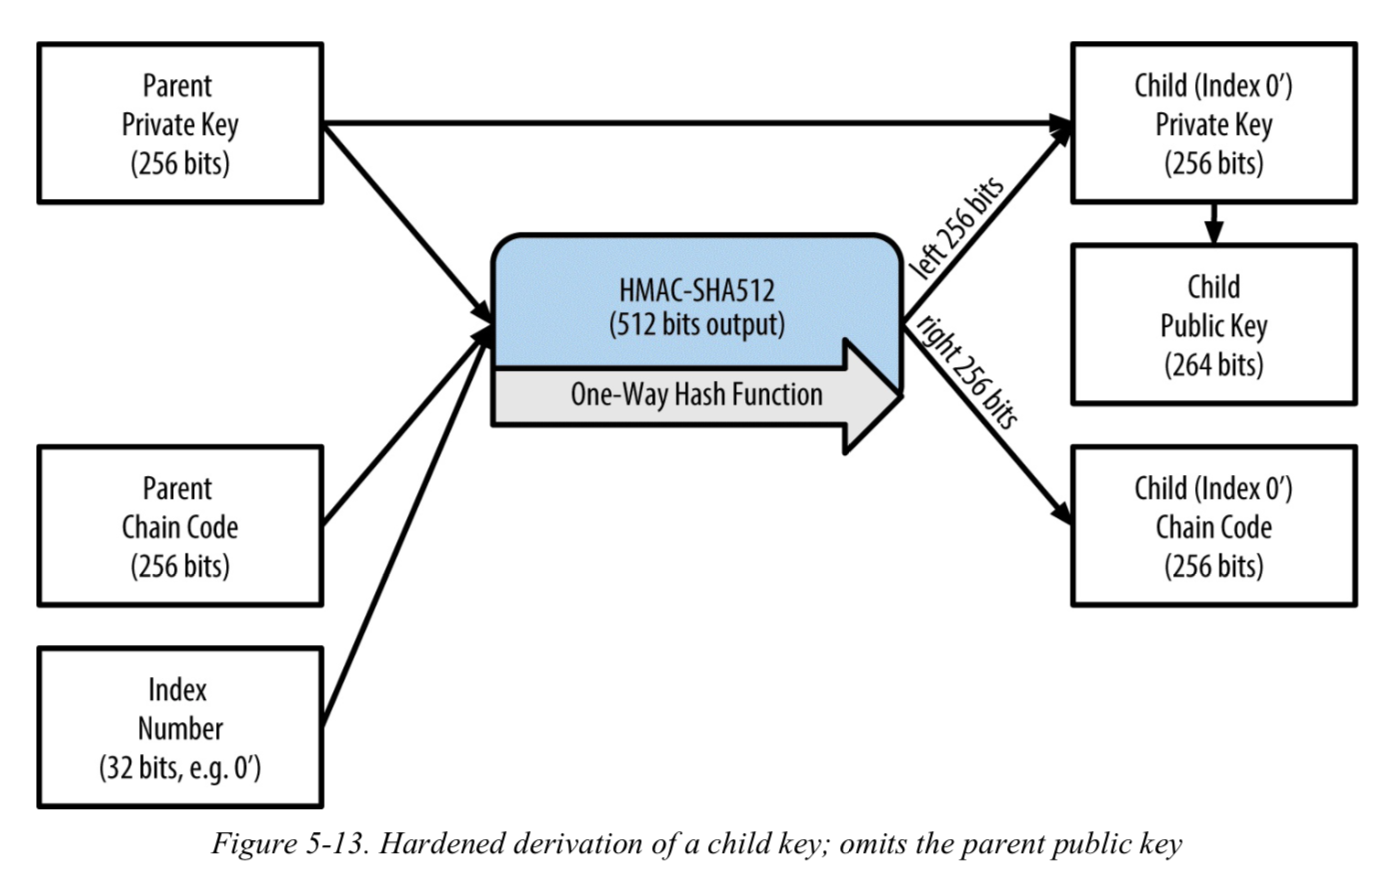
\includegraphics[width=.7\textwidth]{./CKDpriv2.png}
%\caption{Hardened child 的派生过程(图片来自《Master Bitcoin》)}\label{fig-parsesig}
%\end{figure}

%\subsubsection{父公钥派生子公钥}

%\begin{figure}[h]
%\centering
%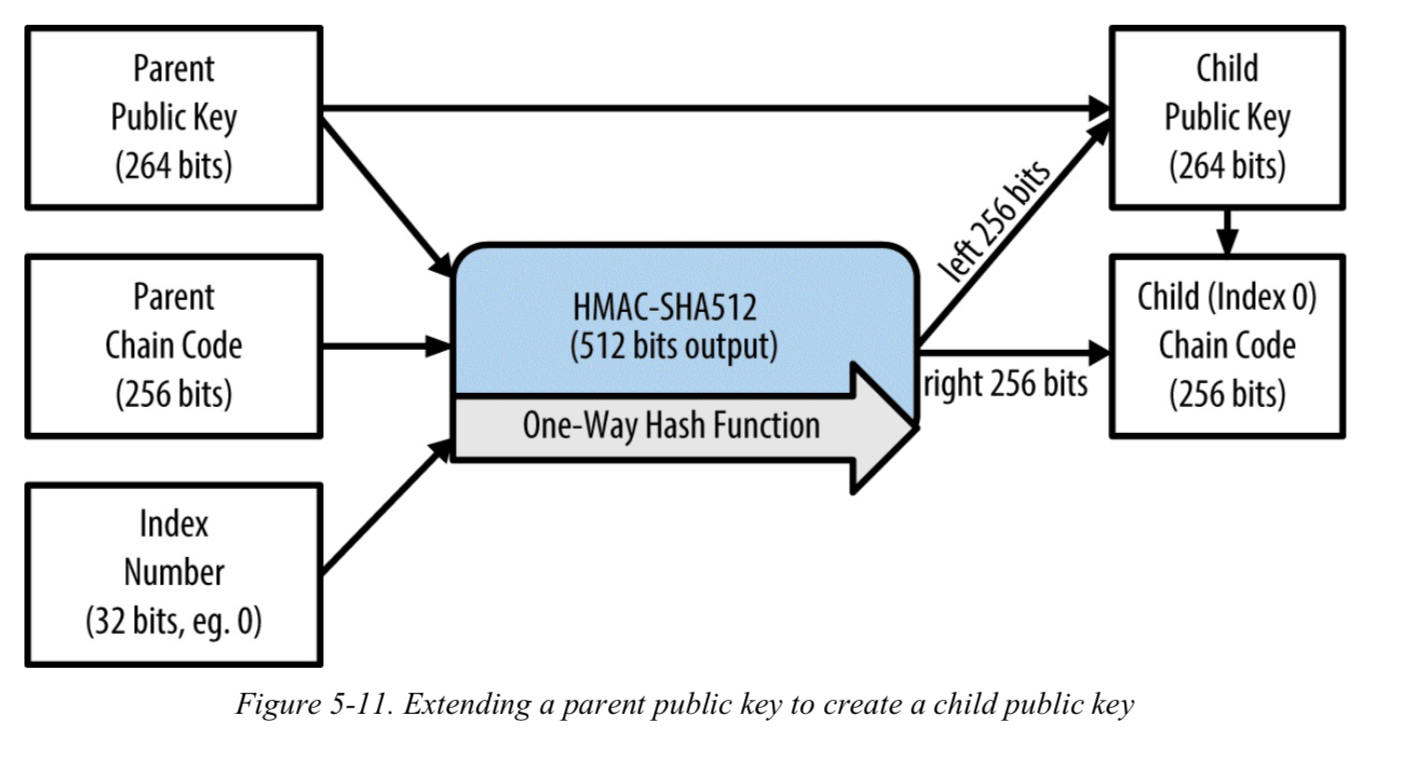
\includegraphics[width=.7\textwidth]{./CKDpub.png}
%\caption{}\label{fig-parsesig}
%\end{figure}

从父公钥派生子公钥的过程在算法~\ref{algo-drc-pub}~中给出,注意该过程只适用于派生平凡子公钥的情形.
从父公钥派生子公钥时, 最终的子公钥$K_i = parse_{256}(I_L) + K_{par}$.

\begin{algorithm}[h]\footnotesize
\caption{子公钥派生算法}\label{algo-drc-pub}
  	\begin{algorithmic}[1]
	    	\STATE 函数$\textsf{CKDpub}((K_{par}, c_{par}), i) \rightarrow (K_i, c_i)$从父扩展公钥计算子扩展公钥
		\STATE 判断索引$i$是否大于等于$2^{31}$, 也即判断子密钥的类型
		\IF {hardened child}
			\STATE return failure  
		\ELSE
			\STATE let $I = \textsf{HMAC-SHA512}(Key = c_{par}, Data = ser_P(K_{par}) || ser_{32}(i))$. 
		\ENDIF
		\STATE 拆分$I$为两个32字节: $I_L || I_R = I, I_L = I[0,\cdots,31], I_R = I[32, \cdots, 63]$.
		\STATE 子公钥$K_i = parse_{256}(I_L) + K_{par}$, 对应的链码为 $c_i = I_R$.
		\STATE 如果$parse_{256}(I_L\geq n)$或者 $K_i$为无穷远点,则递增$i$重新计算
    \end{algorithmic}
\end{algorithm}

椭圆曲线点群上点加法与$\Z_n$上模$n$加法的同态性保证了按照
算法~\ref{algo-drc-pub}~派生而来的子公钥与算法~\ref{algo-drc-priv}~中根据相同索引派生出的子私钥是一一对应的.
这也就是在计算平凡子密钥时, 平凡子公钥和平凡子私钥的派生可以分开独立进行的原因.
记$E(\F_p)$为基于有限域$\F_p$, 基点为$G$, 阶数为$n$的椭圆曲线点群, 
则存在一个从$\Z_n$到$E(\F_p)$的映射$f(x)=xG, x\in\Z_n$,并且该映射$f$是保持加法操作的:
即对于$\Z_n$上的任意值$x$, 都有
$$ f(x+\Delta_x)=f(x)+f(\Delta_x) \Leftrightarrow (x + \Delta_x)G = xG + \Delta_xG, \text{其中}\ \Delta_x \in \Z_n.$$ 
把上式中的$x$当做父私钥, 而$\Delta_x$当做$\textsf{HMAC-SHA512}$输出的$I_L$,
则$f$即为从私钥计算相应公钥的过程.
这也就是说,将私钥$x$先加上一个偏移量$\Delta_x$,再通过$f$变换得到的结果,
与先将私钥$x$和偏移$\Delta_x$映射到公钥,再做加法得到的结果是相同的.


\begin{figure}
\centering
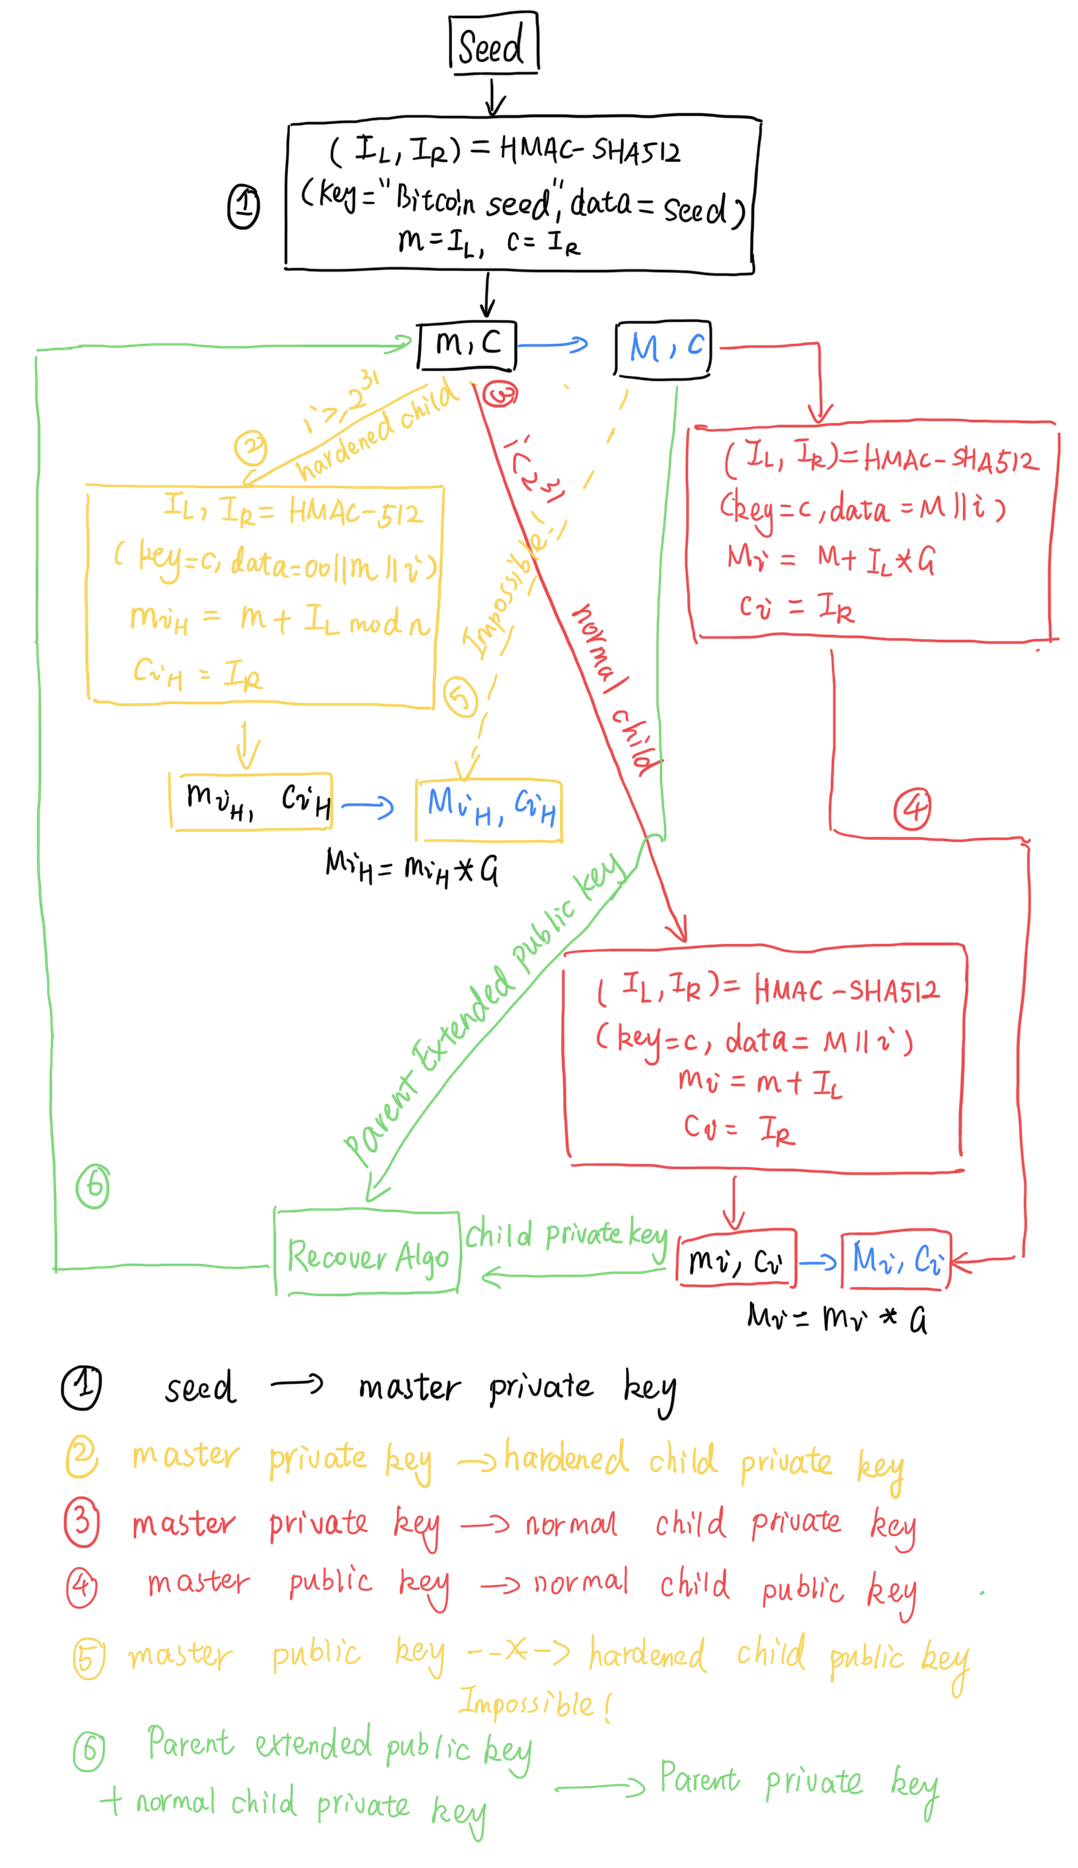
\includegraphics[width=.7\textwidth]{./outline.png}
\caption{分层确定性钱包密钥派生原理}\label{fig-bip32}
\end{figure}


根据算法~\ref{algo-drc-priv}~和算法~\ref{algo-drc-pub}~可知,有两种方式从父私钥派生子公钥.
可以先根据算法~\ref{algo-drc-priv}~从父私钥派生出子私钥然后得到子公钥:
$$k_i, c_i = \textsf{CKDpriv}((k_{par}, c_{par}), i),\ K_i = k_iG.$$
也可以先根据父私钥计算父公钥,然后根据算法~\ref{algo-drc-pub}~得到子公钥
$$K_{par} = k_{par}G,\ K_i, c_i = \textsf{CKDpub}((K_{par}, c_{par}), i).$$ 
如前所述,算法~\ref{algo-drc-pub}~只适用于平凡子密钥派生的情形.

根据算法~\ref{algo-drc-priv}~和算法~\ref{algo-drc-pub}~可知, 可以从一个扩展密钥出发,
逐层派生出一棵密钥树,通常称这个扩展密钥为扩展主密钥.
扩展主密钥通常不是直接生成的,而是从一个可能更短的种子派生而来.
BIP-32中给出了具体的计算步骤.
首先利用密码学安全的的伪随机数发生器(Cryptographically Secure Pseudo-Random Number Generator)生成种子$Seed$.
种子的比特长度通常介于128比特到512比特之间,推荐使用256比特.然后执行如下计算:
$$I = \textsf{HMAC-SHA512}(Key = ``Bitcoin seed", Data = Seed),$$
将$I$划分$I_L = [0,\cdots,31], I_R = [32,\cdots,63]$,
则扩展主私钥为$I_L$, 主链码(Master Chain Code)为$I_R$.
有了扩展主密钥之后,就可以根据算法~\ref{algo-drc-priv}~和算法~\ref{algo-drc-pub}~逐层派生密钥树.
密钥派生的整体结构图参见Figure~\ref{fig-bip32}~,其中绿色表示Recover算法, Section~\ref{sec-security}~中具体阐述.



\subsection{BIP44: 分层确定性钱包的逻辑分层}

为了方便标记和说明, 将$\CKDpriv (\CKDpriv (\CKDpriv (m,3_H),2),5)$记为 $m/3_H/2/5$,
将$\CKDpub (\CKDpub (\CKDpub (M,3),2),5)$记为$M/3/2/5$.其中$m$代表主私钥, $M$代表主公钥.
BIP44对确定性钱包的逻辑层次做了如下限定:
$$m / \text{purpose}' / \text{coin-type}' / \text{account}' / \text{change} / \text{address-index},$$
其中符号$'$代表了这一层使用的是增强子密钥的派生方式. 
purpose字段设定为常量$44‘$,代表了逻辑分层符合BIP44规范;
coin-type字段用于表示不同的数字货币, 从而根据数字货币种类对密钥空间进行划分,
对于一种数字货币而言该字段为一个常量,开发者需要为他们的数字货币申请尚未使用的值;
account字段用于根据不同的用户身份和使用目的对密钥空间进行划分,允许钱包将不同账户隔离开来,
字段值从0 开始递增,在当前账户没有任何交易历史的情况下,钱包软件应当阻止新账户的生成,
并且在用户从外部导入种子后,钱包需要恢复所有已经使用过的账户;
change字段为$0$代表外部的密钥链,也即暴露给其他人用来收款的地址,
值为$1$则代表内部的密钥链,对于外部是不可见的,如用作找零地址等;
address-index字段从0开始连续递增,该索引即为BIP32中定义的用于派生子密钥的索引值.

\begin{table}[h]
\centering
\caption{\textbf{数字货币的密钥分层示例}}
\begin{tabular}{|c|c|c|c|c|}
\hline
\small
Coin &  Account  &   Chain  &  Address &  Path \\\hline
Bitcoin &  first  &  external &  first &  m/44'/0'/0'/0/0 \\\hline
Bitcoin &  second  &  external &  first &  m/44'/0'/1'/0/0 \\\hline
Bitcoin &  first  &  change &  first &  m/44'/0'/0'/1/0 \\\hline
Bitcoin &  first  &  external &  second &  m/44'/0'/0'/0/1 \\\hline
Bitcoin Testnet &  first  &  external &  first &  m/44'/1'/0'/0/0\\\hline
\end{tabular}
\end{table}

前面已经提及到, HD钱包的优势在于将很多私钥的管理简化对种子的管理,尤其是进行导入导出时只需要导出导入种子.
钱包方面需要根据用户导入的种子值,对用户使用过的账户进行恢复.具体步骤如下:
\begin{enumerate}
\item 派生第一个账户节点(index = 0)。
\item 派生该账户的外部链节点。
\item 根据下述的gap limit对外部链进行扫描。
\item 如果该外部链的地址上没有发生过交易,则停止扫描。
\item 反之,递增账户的索引序号,并重复上述步骤1。
\end{enumerate}
Gap limit目前被设置为20,即当扫描到某个账户的外部链中有连续20个没有被使用的地址时,就停止扫描.
该算法有效的前提是,存在账户没有被使用时,钱包需要阻止用户通过递增索引继续生成下一个新账户,
并且在同一个账户下,存在20个连续的地址没有被使用时,阻止用户跨越这些地址生成下一个新地址.

\subsection{安全性分析}\label{sec-security}

分层确定性钱包的密钥派生方案能够保证给定一个公钥$K$,
攻击者计算出相应私钥$k$的难度至少和椭圆曲线点群上的离散对数问题一样难
,这是由基于椭圆曲线的密码学方案所提供的.
通过给定的扩展子私钥$(k_i,c_i)$和索引值$i$恢复父私钥$k_{par}$的难度
至少和攻击\textsf{HMAC-SHA512}一样难,而\textsf{HMAC-SHA512}提供了256比特的安全强度.
判断给定的$N$个(索引, 扩展子私钥)对$(i_j, (k_j, c_j)), 0\leq j \leq N, 2\leq N \leq 2^{32}-1$
是否由同一个扩展父私钥派生而来,至少和攻击\textsf{HMAC-SHA512}一样难,也是不现实的.

给定一个扩展父公钥$(K_{par},c_{par})$ 和一个平凡子公钥$K_i$, 找到该子公钥对应的索引$i$是容易的.
平凡子密钥的索引值$i$的取值范围为$0\leq 0\leq2^{31}-1$,在前述条件下,
可以遍历$i$来重复子公钥的派生的过程,并比较派生出的子公钥是否与给定的子公钥相等.
如果相等,则$i$就是该子公钥对应的索引值.

给定一个扩展父公钥$(K_{par},c_{par})$和平凡子私钥$(k_i)$, 计算父私钥$k_{par}$是容易的.
很容易根据平凡子私钥计算平凡子公钥,则根据前述说明,很容易计算出该子密钥对应的索引值$i$.
由于$I = \textsf{HMAC-SHA512}(Key = c_{par}, Data = ser_P(K_{par}) || ser_{32}(i))$, 
并且有$I_L = I[0,\cdots,31], \ I_R = I[32,\cdots,63]$以及$k_i \equiv parse_{256}(I_L) + k_{par} \mod n$.   
则 $k_{par} \equiv k_i-parse_{256}(I_L)\mod n.$

Listing~\ref{lst-recover}~中的代码展示是前述攻击过程的PoC示例,代码基于分层确定性钱包的Python实现库
bip32utils\footnote{\url{https://github.com/lyndsysimon/bip32utils}}.

\begin{lstlisting}[language=python, caption=基于父扩展公钥和平凡子私钥恢复父私钥的攻击示例, label=lst-recover]
CURVE_GEN  = ecdsa.ecdsa.generator_secp256k1
CURVE_ORDER  = CURVE_GEN.order()
BIP32_HARDEN = 0x80000000 
def recover_parent_privkey(parent_pubkey,child_privkey):
	# traverse all possible non-hardened child index (0~2^31-1) to 
	find the corresponding index of child_privkey
	for i in xrange(0, BIP32_HARDEN +1):
		child=parent_pubkey.CKDpub(i)
		if(child.PublicKey()==child_privkey.PublicKey()):
			break
    # if i is larger than 2^31-1, means that it corresponds to a hardened child, 
    then the recovery is impossible
	if i & BIP32_HARDEN:
		print "can not recover parent private key with a hardened child node"
		return
	# data is composed of public key || i
	data=parent_pubkey.PublicKey()+struct.pack(">L",i)
	(Il,Ir)=parent_pubkey.hmac(data)
	Il_int = string_to_int(Il)
	if Il_int > CURVE_ORDER:
	    return None
	cpk_int=string_to_int(child_privkey.k.to_string())
	# recover parent private key ppk_int from cpk_int= ppk_int + Il_int mod n
	ppk_int=(cpk_int-Il_int)%CURVE_ORDER
	return int_to_string(ppk_int).encode('hex')
\end{lstlisting}

按照BIP32\footnote{
\url{https://github.com/bitcoin/bips/blob/33e040b7bdf5d937599d2401454878d6293476c9/bip-0032.mediawiki\#Test_vector_2}}
测试向量2中给定的seed,
计算出相应路径下的child private/public key,按照上述算法
\ref{lst-recover},通过调用\textsf{recover_parent_privkey(M,m/0)}可成功恢复M的私钥m。

这对于分层确定性钱包的安全性有重要影响,因为这意味着知道一个扩展父公钥和平凡子私钥,
就可以推算出父私钥. 因此管理扩展公钥需要比通常的公钥更为谨慎.
对于采用增强方式派生的密钥则不存在上述问题,因为增强密钥只能通过扩展父私钥派生而来.
这也是在BIP44中规定在purpose, coin-type, account层使用hardened 节点的原因,
以防止这三层上一层的私钥被攻击者按照前述程恢复出来.





\section{BIP39: 从助记词生成确定性密钥}

BIP39提出了一种从助记词(Mnemonic Code)派生HD钱包种子的方法,
使得用户只需要掌握这组助记词即可借助钱包实现派生出HD钱包的密钥树,从而优化用户的交互体验.  
该协议主要包含两个过程: 从熵值(Entropy)生成助记词的过程以及从助记词派生种子的过程.
其中,助记词是从事先定义好的单词列表(Wordlist)里选出的符合相应长度要求的单词集合,
目前针对英语, 日语, 韩语, 西班牙语, 中文(简体/繁体), 法语, 意大利语都有相应的单词列表,
在使用前都对它们进行UTF-8编码处理,详见单词列表\footnote{
Wordlists. \url{https://github.com/bitcoin/bips/blob/master/bip-0039/bip-0039-wordlists.md}}.

用来产生助记词的熵值的比特长度为128到512比特,要求长度必须是32比特的整数倍.
熵值的比特长度越大,安全性就越高,但同时生成助记词中单词的个数也越多.
助记词的产生过程: 假设初始的熵值为$e$, 比特长度为$\textsf{bits}(e)$,
取$\textsf{SHA256}(e)$的前$\textsf{bits}(e)/32$比特作为检验和(Checksum)缀在$e$的后面,
随后将级联后的比特串以11比特为单位进行分组,即每个分组的数字范围是为$[0,\cdots,2047]$,
将其作为索引从单词列表中读取相应的单词,最终选出的词语即构成了一个助记词句子(Mnemonic Sentence).
当$\textsf{bits}(e)=128,192,256$时,对应的助记词的个数为12, 18, 24.
参见Figure~\ref{fig-entropy2mnemonic}(截取自``Mastering Bitcoin 2nd Edition - 
Programming the Open Blockchain''\footnote{
\url{https://github.com/bitcoinbook/bitcoinbook}}).

\begin{figure}[h]
\centering
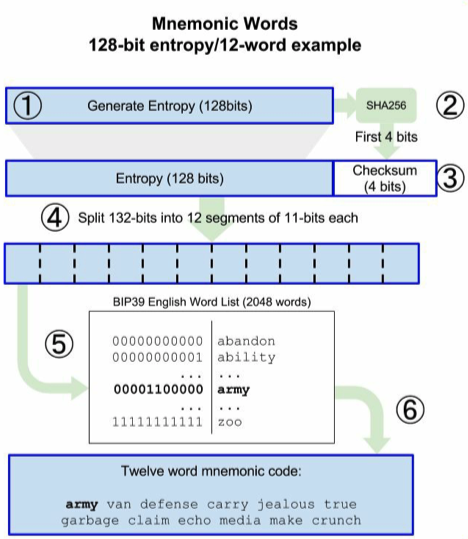
\includegraphics[width=.5\textwidth]{./entropy2mnemonic.png}
\caption{从熵值生成助记词}\label{fig-entropy2mnemonic}
\end{figure}

%下面的列表展示了初始熵值长度ENT,校验和长度与生成的mnemonic sentence长度之间的关系:
%		$$CS = ENT / 32$$
%		$$MS = (ENT + CS) / 11$$
%\begin{table}[h]
%\centering
%\begin{tabular}{|c|c|c|c|c|}
%\hline
%\small
%ENT &  CS  &   ENT+CS  &  MS  \\\hline
%128 &  4  &  132 &  12  \\\hline
%160 &  5  &  165 &  15 \\\hline
%192 &  6  &  198 &  18 \\\hline
%224  &  7  &  231 &  21 \\\hline
%256  &  8  &  264 &  24 \\\hline
%\end{tabular}
%\end{table}

BIP39规定使用\textsf{PBKDF2}函数从助记词生成种子, \textsf{PBKDF2}各参数设置如下:
助记词以UTF-8 NFKD (UTF-8 using Normalization Form Compatibility Decomposition)编码后作为$P$,
``mnemonic''级联$P$同样使用UTF-8 NFKD进行编码后作为盐值$S$,
$c=2048,\ PRF=\textsf{HMAC-SHA512},\ dklen=512$.
最终该算法输出的512比特作为分层确定性钱包的种子.
Listing~\ref{lst-seed}~中的代码基于Trezor的python-mnemonic库\footnote{
\url{https://github.com/trezor/python-mnemonic}}:

\begin{lstlisting}[language=python, caption=基于助记词句子的种子派生, label=lst-seed]
def seed_derivation_from_mnemonic():
    import binascii
    import sys
    from bip32utils import BIP32Key
    if len(sys.argv) > 1:
        data = sys.argv[1]
    else:
        data = sys.stdin.readline().strip()
    data = binascii.unhexlify(data)
    m = Mnemonic('english')
    code=m.to_mnemonic(data)
    seed=m.to_seed(code,'TREZOR')
    xprv = BIP32Key.fromEntropy(seed).ExtendedKey()
    print('mnemonic : %s (%d words)' % (code, len(code.split(' '))))
    print('seed     : %s (%d bits)' % (binascii.hexlify(seed),len(seed) * 4))
    print('xprv     : %s' % xprv)
\end{lstlisting}

\begin{lstlisting}[language=bash, caption = Listing~\ref{lst-seed}~的执行结果示例]
mnemonic : void come effort suffer camp survey warrior heavy shoot primary clutch crush open amazing screen patrol group space point ten exist slush involve unfold (24 words) 

seed : 01f5bced59dec48e362f2c45b5de68b9fd6c92c6634f44d6d40aab69056506f0e35524a    518034ddc1192e1dacd32c1ed3eaa3c3b131c88ed8e7e54c49a5d0998 (256 bits) 

xprv : xprv9s21ZrQH143K39rnQJknpH1WEPFJrzmAqqasiDcVrNuk926oizzJDDQkdiTv
       NPr2FYDYzWgiMiC63YmfPAa2oPyNB23r2g7d1yiK6WpqaQS
\end{lstlisting}

\section{BIP38: 基于口令保护私钥}

BIP38提出了基于口令(Passphrase/Password)对私钥进行加密保护的方案.
该方案只考虑了针对私钥的机密性保护,而没有考虑提供完整性保护(从密码学角度来讲不算是最佳实践),
因此其主要针对纸钱包(Paper Wallet)等私钥密文不容易遭受篡改的应用场景.
BIP38中给出了两种加密私钥的方法,其中一种方法使用了EC乘法操作,
另一种没有使用EC乘法操作.两种方法实现的功能有很大的区别.
方便起见,后续我们用方法一指代没有使用EC乘法操作的加密方法,用方法二指代使用了EC乘法操作的加密方法.

未使用EC乘法操作的方法一中, 对于已经产生的私钥, 使用用户设置的口令对私钥进行加密.
加密后的密文与口令在解密私钥时缺一不可.由于两者可以独立管理,可以提高私钥的安全性.

使用了EC乘法操作的方法二中, 用户首先会生成一个中间口令码(Intermediate Passphrase Code),
%(包含一个由passphrase单向生成的椭圆曲线群上的点,以及用户产生的salt),
并将其传输给一个第三方.
%(由于该方案针对的场景主要是纸钱包,这里的第三方通常是一个printer),
第三方可以为用户生成新的地址,并将新地址和计算地址对应的私钥所必须的信息发给用户
%并对恢复该地址对应私钥的必要信息加密后展示给用户.
用户拿到前述信息后结合口令,即可算出新地址对应的私钥.
这种方式允许用户将生成新地址的工作委托给无需可信的第三方来做,但同时保证只有知道口令和密文的人才能计算出对应私钥.

%BIP38同时给出了对应于两种方法的密文数据编码方式,虽然格式不同,但长度都为39个字节.
%方法一中最终的密文数据为以下字节序列\textsf{Base58Check}编码:
%$$0x01 || 0x42 || flagbyte || addrhash || encryptedhalf_1 || encryptedhalf_2.$$
%方法二中最终的密文数据为以下字节序列的\textsf{Base58Check}编码:
%$$0x01 || 0x43 || flagbyte || addrhash || ownerentropy || encryptedhalf_1 || encryptedhalf_2.$$
%
%\begin{itemize}
%\item 对于不使用EC乘法的,最终的数据由对$0x01 \ 0x42+ flagbyte+ addrhash+ encryptedhalf1 + encryptedhalf2$
%进行Base58Check编码后的数据构成.而对于使用EC乘法的,加密保护后的私钥数据由
%$0x01 \ 0x43+ flagbyte+ addrhash+ ownerentropy+ encryptedhalf1 \  + encryptedhalf2$
% 进行Base58Check编码后的数据构成(具体含义会在后面详细介绍).
%
%\item $0x01\ 0x42/43$是为了使经过Base58Check编码后的结果以$6P$开头,
%6代表了"a private key that needs something else to be usable",P代表了上一句中的"something is a passphrase".
%
%\item flagbyte为1字节,最高两位用来区分是否使用EC乘法:
%11表示不使用EC乘法,反之设置为00.$0x20$用来表示私钥转换成比特币地址时使用的是压缩公钥的格式.
%$0x40$用来表示在使用EC乘法时,同时也使用了lot+sequence,这两个数字的作用会在后面说明.$0x10,0x08$予以保留.
%
%\item Addrhash为对比特币地址进行两次SHA256操作后,取前四个字节的结果.
%\end{itemize}

\subsection{不使用EC乘法的加密方法一}

该方法对已有私钥$k$进行加密,加密过程分为两步:用Scrypt算法从口令$P$
派生AES算法加密所需密钥;使用AES算法对私钥信息进行加密.
记该私钥对应的Bitcoin地址为$address$, 按照以下Algorithm~\ref{algo-m1}~展示的步骤进行.

\begin{algorithm}[h]\footnotesize
\caption{不使用EC乘法的加密方法一}\label{algo-m1}
\begin{algorithmic}[1]
	    	\STATE 计算地址哈希值 $addresshash = \textsf{SHA256}(\textsf{SHA256}(address))[0,1,2,3]$
		\STATE 用Scrypt根据口令等派生64字节值$v=v_1||v_2, v_1 = v[0,\cdots, 31], v_2= [32,\cdots,63]$
		\STATE 计算$ek_1 = \textsf{AES256Encrypt}(block = k[0...15] \oplus v_1[0,\cdots,15], key = v_2)$
		\STATE 计算$ek_2 = \textsf{AES256Encrypt}(block = k[16...31] \oplus v_1[16...31], key = v_2)$
		\STATE 密文为$0x01 || 0x42 || flagbyte || addrhash || ek_1 || ek_2$的\textsf{Base58CheckEncode}
\end{algorithmic}
\end{algorithm}


%\begin{enumerate}
%\item 计算地址哈希值 $addresshash = \textsf{SHA256}(\textsf{SHA256}(address))[0,1,2,3]$
%\item 用Scrypt根据口令等派生32字节值$v=v_1||v_2, v_1 = v[0,\cdots, 31], v_2= [32,\cdots,63]$
%\item 计算$ek_1 = \textsf{AES256Encrypt}(block = k[0...15] \oplus v_1[0,\cdots,15], key = v_2)$
%\item 计算$ek_2 = \textsf{AES256Encrypt}(block = k[16...31] \oplus v_1[16...31], key = v_2)$
%\item 密文为$0x01 || 0x42 || flagbyte || addrhash || ek_1 || ek_2$的\textsf{Base58Check}编码
%\end{enumerate}


\begin{figure}[h]
\centering
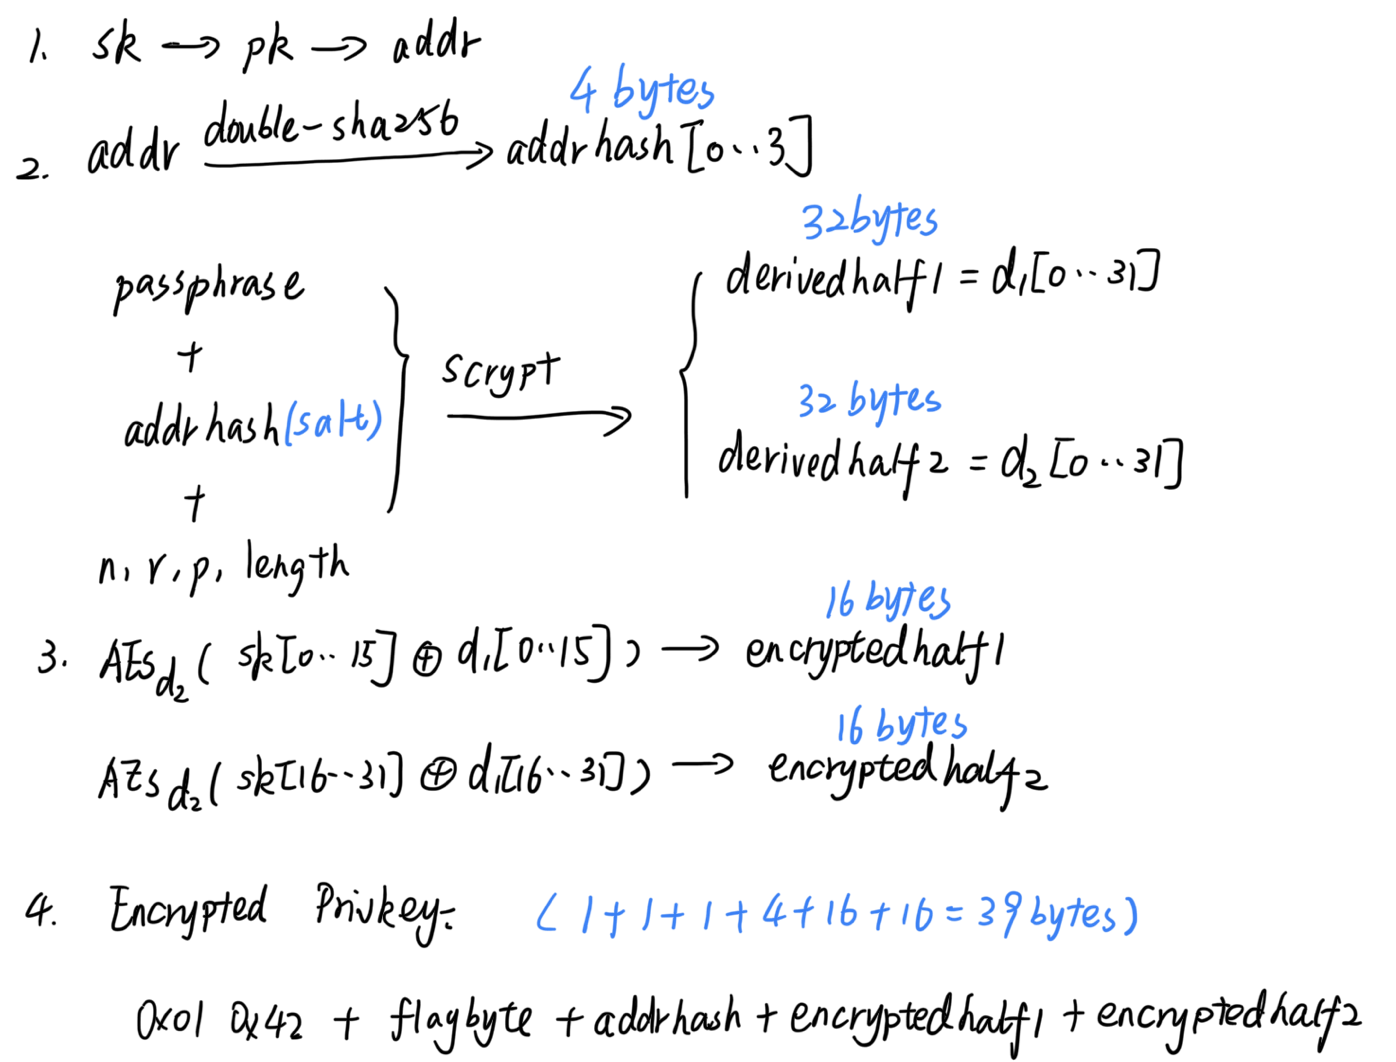
\includegraphics[width=.7\textwidth]{./no-ec.png}
\caption{不使用EC乘法的加密方法一: 加密过程}\label{fig-m1-enc}
\end{figure}

在使用Scrypt派生密钥时, 参数$P$为用UTF-8编码并用NFC (Unicode Normalization Form C)正则化后的口令,
$S$设置为$addresshash$,也即$ \textsf{SHA256}(\textsf{SHA256}(address))$的前4个字节, 
该字段无需保密,目的是为了引入更多的熵值,以增加攻击者进行暴力破解时的搜索空间.
$n, r, p$的值为系统设置参数,并且$n=16384,\ r=8,\ p=8,\ length=64$.
最终的密文为39个字节,参见Figure~\ref{fig-m1-enc}.
其中$flagbyte$为1个字节,最高两位用来区分是否使用EC乘法:
$flagbyte_{7,6}=11$表示不使用EC乘法,
$flagbyte_{7,6}=00$表示使用了EC乘法.
比特$flagbyte_{5}=1$表示使用比特币地址是根据压缩形式的公钥计算而来的,
注意Bitcoin中同一个私钥可以有两种比特币地址,分别对应压缩形式公钥和不压缩形式公钥.
$flagbyte_{2}=1$表示在使用EC乘法加密时还使用了lot+sequence字段,这两个字段的作用会在后面说明.
其余比特位保留.

%\begin{algorithm}[h]\footnotesize
%\caption{Encryption}\label{encryption without ec multiply}
%  	\begin{algorithmic}[1]
%	    \STATE 计算Bitcoin地址(ASCII), 计算addresshash,也即地址哈希值$\textsf{SHA256(SHA256())}$的前4个字节
%		\STATE 用scrypt从口令派生密钥
%	⁃	
%		\STATE 参数: passphrase 是用UTF-8编码并用NFC (Unicode Normalization Form C)正则化后的值. 
%		salt 是之前计算的addresshash, $n=16384, r=8, p=8, length=64 $(n, r, p are provisional and subject to consensus)  
%		\STATE Let's split the resulting 64 bytes in half, and call them derivedhalf1 and derivedhalf2
%		\STATE Do $encryptedhalf1 = \textsf{AES256Encrypt}(block = bitcoinprivkey[0...15] \oplus derivedhalf1[0...15], key = derivedhalf2)$,
%		\STATE Do $encryptedhalf2 = AES256Encrypt(block = bitcoinprivkey[16...31] \oplus derivedhalf1[16...31], key = derivedhalf2)$, 
%		\STATE The encrypted private key is the Base58Check-encoded concatenation of the following, which totals 39 bytes without Base58 %checksum:$0x01$ $0x42 + flagbyte + salt + encryptedhalf1 + encryptedhalf2$
%    \end{algorithmic}
%\end{algorithm}

解密过程首先根据用户掌握的passphrase计算出AES的解密密钥,随后对密文解密,
首先也需要通过Scrypt计算$v_1, v_2$, 然后利用\textsf{AES256Encrypt}解密得到私钥的值,
通过私钥根据$flagbyte$中的信息派生Bitcoin地址,并进一步计算$addresshash$并与密文中的该字段进行对比.
如果不匹配则报告输入的口令错误. 加密和解密的PoC代码实现参见Listing~\ref{lst-m1},
执行结果参见Listing~\ref{lst-m1res}.


%\begin{algorithm}[h]\footnotesize
%\caption{Decryption}
%  	\begin{algorithmic}[1]
%	    \STATE Collect encrypted private key and passphrase from user.  
%		\STATE Derive derivedhalf1 and derivedhalf2 by passing the passphrase and addresshash into scrypt function.
%		\STATE Decrypt encryptedhalf1 and encryptedhalf2 using AES256Decrypt, merge them to form the encrypted private key. 
%		\STATE Convert that private key into a Bitcoin address, honoring the compression preference specified in flagbyte of the encrypted %key record.
%		\STATE Hash the Bitcoin address, and verify that addresshash from the encrypted private key record matches the hash. If not, report %that the passphrase entry was incorrect.  
%    \end{algorithmic}
%\end{algorithm}

\begin{lstlisting}[language=python, caption = 不使用EC乘法的加解密过程示例, label=lst-m1]

import hashlib 
import secrets
from Crypto.Cipher import AES
import base58check
import scrypt
from bitcoinlib.keys import *
import ecdsa
from ecdsa.curves import SECP256k1
from ecdsa.ecdsa import int_to_string, string_to_int

# parameter for Scrypt function
SCRYPT_N=16384
SCRYPT_R=8
SCRYPT_P=8

def b58check(data):
	# return base58 encoding of data with checksum
	checksum=hashlib.sha256(data).digest()
	checksum=hashlib.sha256(checksum).digest()
	data+=checksum[:4]
	return base58check.b58encode(data)

def enc_without_ec_multi(privkey,address,passphrase,compressed):
	# compute addrhash of corresponding address to known private key
	addrhash=hashlib.sha256(address).digest()
	addrhash=hashlib.sha256(addrhash).digest()
	addrhash=addrhash[:4]
	# derive encryption key for AES
	passphrase=passphrase.decode('utf-8')
	d=scrypt.hash(passphrase,addrhash,SCRYPT_N,SCRYPT_R,SCRYPT_P,64)
	derivedhalf1=d[:32]
	derivedhalf2=d[32:64]
	# encryption process
	m1=[a^b for a,b in zip(privkey[:16],derivedhalf1[:16])]
	m2=[a^b for a,b in zip(privkey[16:32],derivedhalf1[16:32])]
	e1=AES.new(derivedhalf2).encrypt(bytes(m1))
	e2=AES.new(derivedhalf2).encrypt(bytes(m2))
   # pack encryption data
	flagbyte=b'\xe0' if compressed==1 else b'\xC0'
	res=b'\x01\x42'+flagbyte+addrhash+e1+e2
	return b58check(res)
	
def dec_without_ec_multi(encrypted_privkey,passphrase):
	# unpack data 
	data=base58check.b58decode(encrypted_privkey)
	addrhash_v=data[3:7]
	passphrase=passphrase.decode('utf-8')
	# derive decryption key for AES
	d=scrypt.hash(passphrase,addrhash_v,SCRYPT_N,SCRYPT_R,SCRYPT_P,64)
	derivedhalf1=d[:32]
	derivedhalf2=d[32:64]
	# decryption process
	m1=AES.new(derivedhalf2).decrypt(data[7:23])
	m2=AES.new(derivedhalf2).decrypt(data[23:39])
	privkey1=bytes([a^b for a,b in zip(m1,derivedhalf1[:16])])
	privkey2=bytes([a^b for a,b in zip(m2,derivedhalf1[16:32])])
	privkey=privkey1+privkey2
	# verify whether addrhash is correct
	k=Key(privkey)
	addr=k.address_uncompressed() if data[2]==0xC0 else k.address()
	addrhash=hashlib.sha256(addr.encode('ascii')).digest()
	addrhash=hashlib.sha256(addrhash).digest()
	if addrhash!=addrhash_v:
		assert("address is not valid!")
	else:
		return privkey1+privkey2
\end{lstlisting}


\begin{lstlisting}[language=bash, caption = Listing~\ref{lst-m1}~的执行结果示例, label=lst-m1res]
Encryption with no EC multiplication:
Privkey is : b'\xcb\xf4\xb9\xf7\x04p\x85k\xb4\xf4\x0f\x80\xb8~\xdb\x90\x86Y\x97\xff\xeem\xf3\x15\xab\x16mq:\xf43\xa5'
Encrypted private key is : b'6PRVWUbkzzsbcVac2qwfssoUJAN1Xhrg6bNk8J7Nzm5H7kxEbn2Nh2ZoGg'

Decryption with no EC multiplication:
Decryption succeed!
Private key is  b'\xcb\xf4\xb9\xf7\x04p\x85k\xb4\xf4\x0f\x80\xb8~\xdb\x90\x86Y\x97\xff\xeem\xf3\x15\xab\x16mq:\xf43\xa5'
\end{lstlisting}


\subsection{使用EC乘法的加密方法二}

该方法利用了EC 乘法的同态性质,主要思想类似于一个基于椭圆曲线的密钥协商方案.
用户事先由口令和熵值等生成一个随机数$x$,并计算对应的椭圆曲线群上的点$P=xG$,将其发给第三方.
随后第三方选择一个随机数$k$与该点进行EC的乘法操作,也即新生成的公钥$P'=kP=(x \cdot k)G$.
随后将$k$加密后发送给用户(加密过程与方法一中类似).
用户收到数据解密后,计算出新私钥$x\cdot k$.
假设用于生成$x$的口令没有泄露,则用户就可以确认新私钥是足够安全的(只有知道口令的人才能计算出新私钥), 
%这一点可以认为是使用该方法生成新的加密私钥所额外带来的一个安全性方面的好处.
方法二主要包括两个阶段:初始化阶段和私钥生成阶段.

初始化阶段主要功能是用户利用口令和熵值计算中间口令码(Intermediate Passphrase Code)并发送给第三方.  
在计算时,用户可以选择性的生成一个20比特的批号(Lot Number)和12比特的序列号(Sequence Number).
在用户向第三方请求大量的加密私钥时,需要检查返回的私钥对应的批号和序列号与用户自己提供的中间口令码中的一致.
4个字节批号和序列号并不是必须的.根据是否使用这两个字段,初始化阶段稍微不同. 
 
 
 在使用批号和序列号时, 按照Algorithm~\ref{algo-m2initwithlnsn}~中的步骤进行初始化. 
 其中第3步中Scrypt输入参数中的$P$为UTF-8编码的并用NFC形式正则化后的用户口令,
 盐值$S$为第1步中生成的$ownersalt$,  $n=16384, r=8, p=8, length=32$.
 第5步中的点的压缩表示形式约束仅限于这一步的计算, 与生成Bitcoin地址时使用的公钥的表示形式无关.
 
\begin{algorithm}[h]\footnotesize
\caption{使用批号和序列号时的初始化阶段}\label{algo-m2initwithlnsn}
  	\begin{algorithmic}[1]
	   	 \STATE 生成4个字节的随机数$ownersalt$
		\STATE 批号和序列号用大端法形式的4字节的整数$lotsequence=lotnumber * 4096 + sequencenumber$
		\STATE  用Scrypt从口令等信息派生32字节密钥$prefactor$
		\STATE 计算$passfactor = \textsf{SHA256}(\textsf{SHA256}(prefactor || ownerentropy))$
		\STATE 计算 $passfactor * G$, 该点的压缩表示形式记为$passpoint$
		\STATE 传送$ownerentropy = ownersalt || lotsequence$以及$passpoint$给第三方
    \end{algorithmic}
\end{algorithm}

 \begin{figure}[h]
\centering
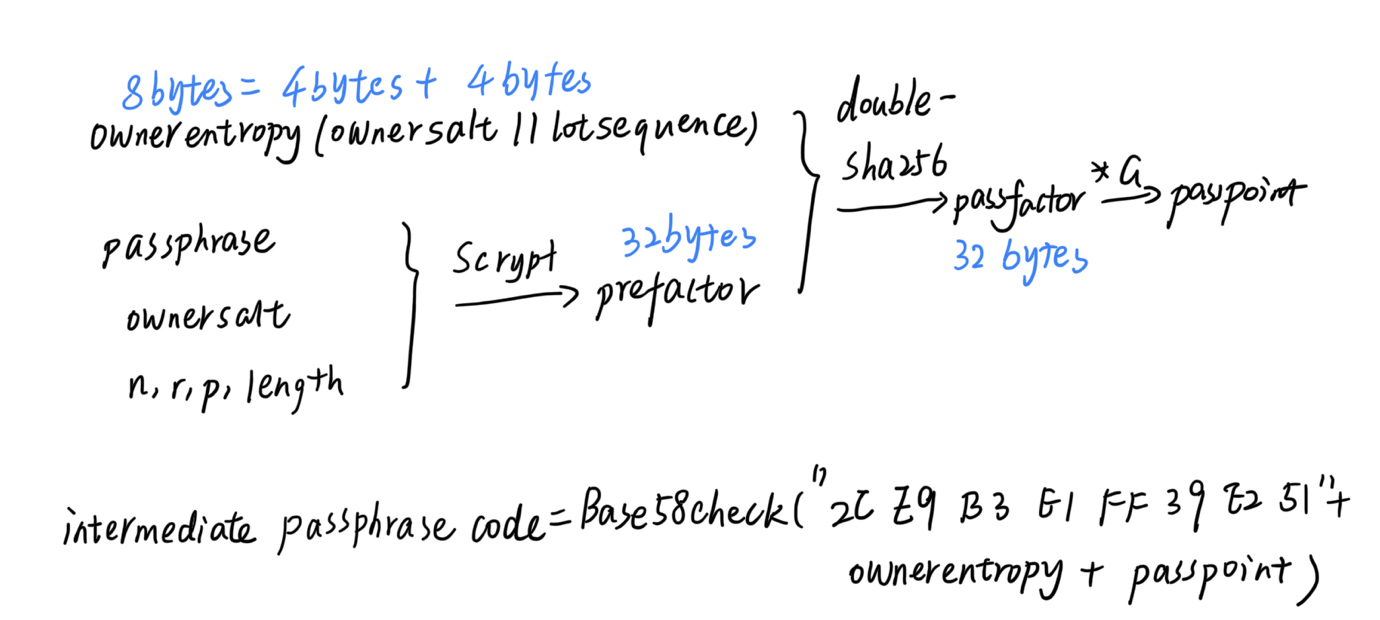
\includegraphics[width=.7\textwidth]{./im-code1.png}
\caption{使用批号和序列号时方法二的初始化过程}\label{fig-m2initwithlnsn}
\end{figure}
 
最后一步中真正发送给第三方的是下面名为\textit{intermediate_passphrase_string}的字符串
(也就是前述的中间口令码):
$$\textsf{Base58CheckEncode}(\textit{2C E9 B3 E1 FF 39 E2 51} || ownerentropy || passpoint)$$
由于魔数(Magic Number) ``2C E9 B3 E1 FF 39 E2 51"的采用,
编码之后的字符串会以``passphrase"开头. 
72个字符的\textit{intermediate_passphrase_string}编码了49个字节的信息以及校验码
49个字节的信息包括8字节的魔数, 8字节的\textit{ownerentropy}以及33字节的\textit{passpoint}.
参见Figure~\ref{fig-m2initwithlnsn}.
 
 
\begin{figure}[h]
\centering
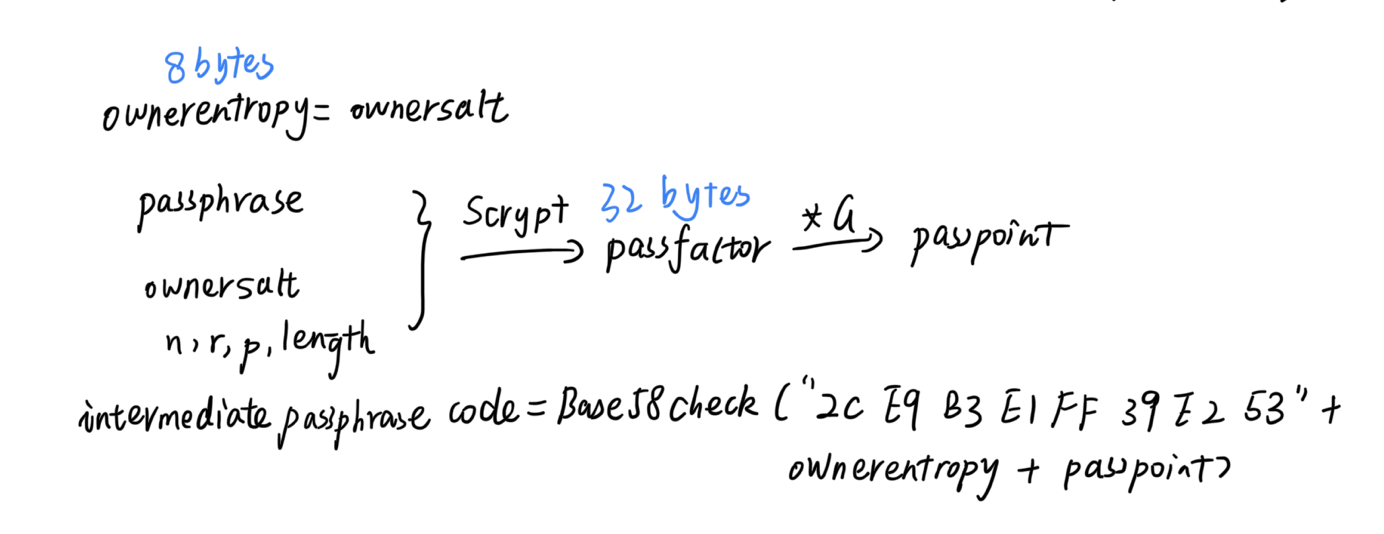
\includegraphics[width=.7\textwidth]{./im-code2.png}
\caption{不使用批号和序列号时方法二的初始化过程}\label{fig-m2initnolnsn}
\end{figure}

 不使用批号和序列号时的初始化过程相对简单. 
 首先生成8字节的随机数$ownersalt$而不是Algorithm~\ref{algo-m2initwithlnsn}~中的4个字节.
 略过批号和序列号字段,此时$ownerentropy$是$ownersalt$的别名.
 Algorithm~\ref{algo-m2initwithlnsn}~中的第4步从$prefactor$生成$passfactor$的计算也略过,
 Scrypt的输出直接作为$passfactor$. 
 \textsf{Base58CheckEncode}编码时使用魔数``2C E9 B3 E1 FF 39 E2 53" (最后一个字节从$0x53$变成$0x51$).
 参见Figure~\ref{fig-m2initnolnsn}.
 
%\begin{algorithm}[h]\footnotesize
%\caption{Initialize without lot sequence}
%  	\begin{algorithmic}[1]
%	    \STATE ownersalt is 8 random bytes instead of 4, and lotsequence is omitted. ownerentropy becomes an alias for ownersalt. 
%		\STATE The SHA256 conversion of prefactor to passfactor is omitted. Instead, the output of scrypt is used directly as passfactor.
%		\STATE The magic bytes are "2C E9 B3 E1 FF 39 E2 53" instead (the last byte is 0x53 instead of 0x51). 
%    \end{algorithmic}
%\end{algorithm}

\subsubsection{加密私钥计算}
第三方拿到中间口令码之后,可以用它为用户生成新的加密私钥.
确切地说,第三方可以为用户生成新的公钥,并将计算对应私钥的所需的信息加密后一并发送给用户,
同时拥有口令和密文信息的人才能从中计算出对应的私钥.  

计算时首先需要设置\textit{flagbyte}, 由于使用了EC
乘法,$flagbyte_{7,6}=00$. 如果采用压缩形式的公钥派生Bitcoin地址,则设置$flagbyte_5=1$.
如果字段$ownerentropy$中包含批号系列号字段,则设置$flagbyte_3=1$.
然后生成24个字节的随机数$seedb$,并计算$factorb=\textsf{SHA256}(\textsf{SHA256}(seedb))$.
计算$generatedpubkey = factorb * passpoint$并计算对应的Bitcoin地址
$generatedaddress=\textsf{RIPEMD160}(\textsf{SHA256}(generatedpubkey))[0,\cdots,19]$,
可使用未压缩或者压缩形式的公钥表示,这就是第三方为用户新生成的Bitcoin地址.


%\begin{algorithm}[h]\footnotesize
%\caption{New Public Key Generation}
%  	\begin{algorithmic}[1]
%	    \STATE Set flagbyte.
%	    \STATE Turn on bit 0x20 if the Bitcoin address will be formed 
%	    by hashing the compressed public key (optional). Turn on bit 0x04 
%	    if ownerentropy contains a value for lotsequence.   
%		\STATE Generate 24 random bytes, call this seedb. 
%		Take $SHA256(SHA256(seedb))$ to yield 32 bytes, call this factorb.
%		\STATE ECMultiply passpoint by factorb. Use the resulting EC point 
%		as a public key and hash it into a Bitcoin address using either 
%		compressed or uncompressed public key methodology. 
%		This is the generated Bitcoin address, call it generatedaddress. 
%    \end{algorithmic}
%\end{algorithm}

前述过程完成了新公钥的生成,下面介绍具体的加密过程,
加密过程与方法一中的加密过程类似:
利用Scrypt派生AES的加密密钥,然后对与新公钥关联的$seedb$进行加密.
具体过程在Algorithm~\ref{algo-m2enc}~中给出.

\begin{algorithm}[h]\footnotesize
\caption{使用EC乘法的方法二的加密过程}\label{algo-m2enc}
  	\begin{algorithmic}[1]
	   	\STATE 计算$addresshash=\textsf{SHA256}(\textsf{SHA256}(generatedaddress))[0,1,2,3]$ 
	    	\STATE 用Scrypt从$passpoint$派生32字节值$v=v_1||v_2, v_1 = v[0,\dots, 31], v_2= [32,\dots,63]$
	    	\STATE 计算$ek_1 = \textsf{AES256Encrypt}(block = (seedb[0,\dots,15] \oplus v_1[0,\dots,15]), key = v_2)$
		\STATE 计算$ek_2 = \textsf{AES256Encrypt}(block = ((ek_1[8,\dots,15] || seedb[16,\dots,23])  \oplus v_1[16,\dots,31]), key = v_2)$
		\STATE 密文为$0x01 || 0x43 || flagbyte || addresshash || ownerentropy ||  ek_1[0...7] || ek_2$的 \textsf{Base58CheckEncode}
    \end{algorithmic}
\end{algorithm}

第2步中函数Scrypt的参数$P$为用户提供的33字节的$passpoint$, 
参数$S$为$addresshash || ownerentropy$, $n=1024, r=1, p=1, length=64$.
这里最终数据的格式略有些奇怪,推测是为了方法一中的结果保持长度一致(都是39个字节).
相比较,这里比前面多了一个8字节的$ownerentropy$字段,
\red{因此选取的$seedb$长度也就限制在了24字节 这句怎么理解 跟上一句串不起来},参见Figure~\ref{fig-m2enc}.

%\begin{algorithm}[h]\footnotesize
%\caption{Encryption}
%  	\begin{algorithmic}[1]
%	    \STATE Take the first four bytes of SHA256(SHA256(generatedaddress)) 
%	    and call it addresshas
%	    \STATE Now we will encrypt seedb. Derive a second key from passpoint 
%	    using scrypt 
%		\STATE Parameters: passphrase is passpoint provided from the first 
%		party (expressed in binary as 33 bytes). 
%		salt is addresshash + ownerentropy, $n=1024, r=1, p=1, length=64$. 
%		The "+" operator is concatenation.
%		\STATE Split the result into two 32-byte halves and call them derivedhalf1 
%		and derivedhalf2.
%		\STATE Do $AES256Encrypt(block = (seedb[0...15] \oplus derivedhalf1[0...15]), 
%		key = derivedhalf2)$, call the 16-byte result encryptedpart1
%		\STATE Do $AES256Encrypt(block = ((encryptedpart1[8...15] + seedb[16...23]) 
%		\oplus derivedhalf1[16...31]), key = derivedhalf2)$, call the 16-byte result 
%		encryptedpart2. The "+" operator is concatenation.
%		\STATE The encrypted private key is the Base58Check-encoded concatenation of 
%		the following, which totals 39 bytes without Base58 checksum: 
%		$$0x01 0x43 + flagbyte + addresshash + ownerentropy +  encryptedpart1[0...7] + 
%		encryptedpart2$$
%    \end{algorithmic}
%\end{algorithm}



\begin{figure}[h]
\centering
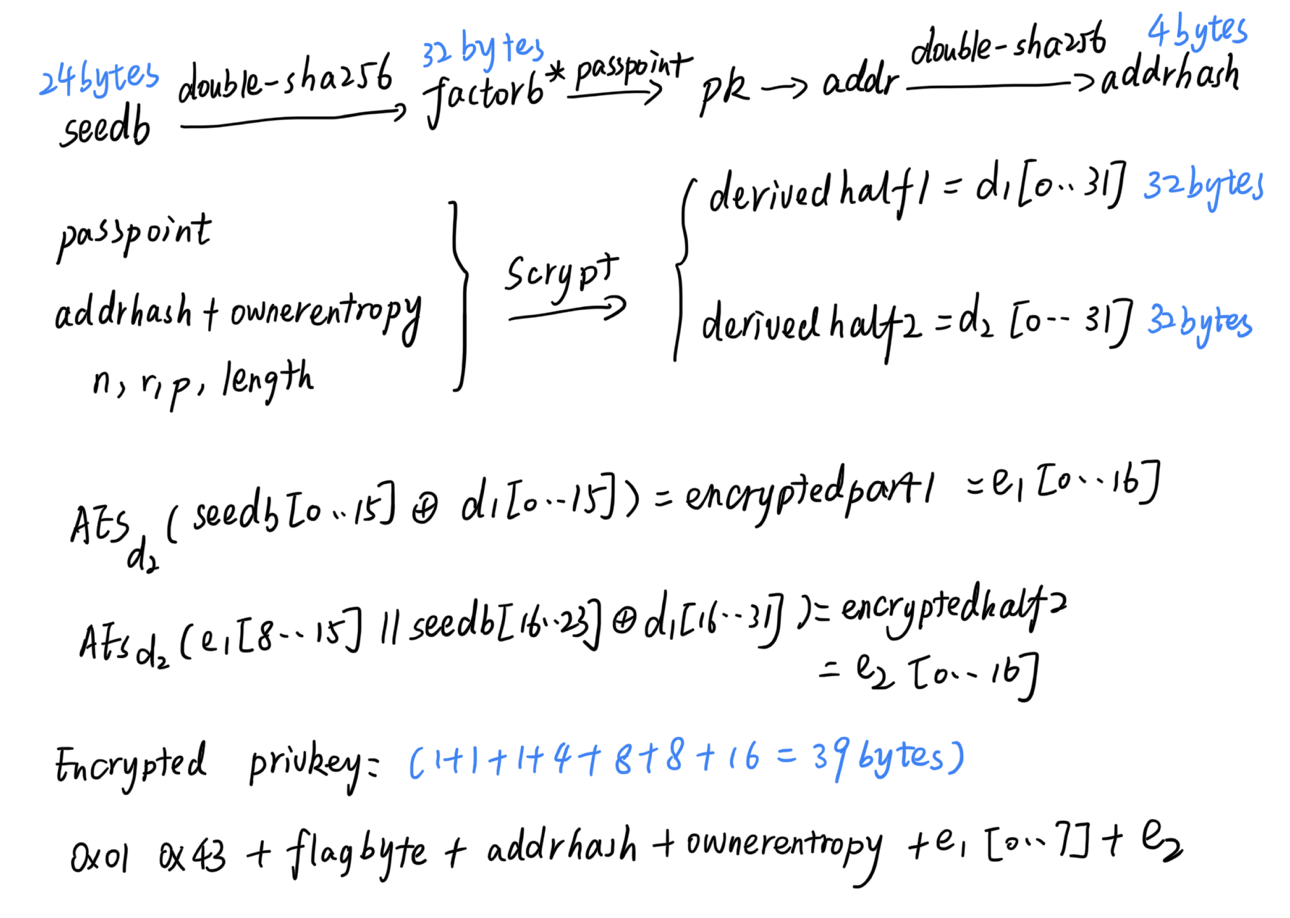
\includegraphics[width=.7\textwidth]{./ec.png}
\caption{使用EC乘法的方法二的加密过程}\label{fig-m2enc}
\end{figure}

\subsubsection{计算新地址对应的私钥}
根据第三方返回的密文计算新私钥的过程在Algorithm~\ref{algo-m2dec}~中展示.
由于新公钥为$passpoint\cdot factorb=passfactor\cdot factorb *G$,
对应的私钥即为$passfactor\cdot factorb$.

\begin{algorithm}[h]\footnotesize
\caption{使用EC乘法的方法二的解密过程与私钥计算}\label{algo-m2dec}
  	\begin{algorithmic}[1]
	   \STATE  用Scrypt函数从$ownersalt$和口令派生$passfactor$并重新计算$passpoint$
	   \STATE 用Scrypt函数从$passpoint, addresshash, ownerentropy$派生$seedb$的解密密钥
		\STATE 用\textsf{AES256Decrypt}解密$ek_2$得到$seedb[16,\dots,23]$和$ek_1[8,\dots,15]$
		\STATE 用\textsf{AES256Decrypt}解密$ek_1$得到$seedb[0,\dots,15]$
		\STATE 用$seedb$计算$factorb$
		\STATE 计算地址$generatedaddress$对应的私钥为$passfactor \cdot factorb$
		\STATE 根据$flagbyte$中的公钥表示形式,从私钥计算对应的Bitcoin地址
		\STATE 根据Bitcoin地址计算$addresshash$并与密文中的字段比较.若不匹配,则口令错误
    \end{algorithmic}
\end{algorithm}

在恢复了新私钥后,客户端还需要验证计算出的私钥与之前$addresshash$给出的地址是否对应,
如果不是,则需要向用户返回错误信息,即用户输入了错误的口令.
由于该协议描述的目的场景是针对纸钱包,所以可假定上述编码后的密文的完整性是保证的.
使用EC乘法的加解密过程示例在Listing~\ref{lst-m2}中给出,执行结果在Listing~\ref{lst-m2res}中给出.
%\begin{algorithm}[h]\footnotesize
%\caption{使用EC乘法的方法二的解密过程与私钥计算}\label{algo-m2dec}
%  	\begin{algorithmic}[1]
%	   \STATE  Collect encrypted private key and passphrase from user.
%	   \STATE  Derive passfactor using scrypt with ownersalt and the user's 
%	   passphrase and use it to recompute passpoint
%	   \STATE Derive decryption key for seedb using scrypt with passpoint, 
%	   addresshash, and ownerentropy
%		\STATE Decrypt encryptedpart2 using AES256Decrypt to yield the last 
%		8 bytes of seedb and the last 8 bytes of encryptedpart1.
%		\STATE Decrypt encryptedpart1 to yield the remainder of seedb.
%		\STATE Use seedb to compute factorb.
%		\STATE Multiply passfactor by factorb mod N to yield the private key 
%		associated with generatedaddress.
%		\STATE C\STATE onvert that private key into a Bitcoin address, honoring 
%		the compression preference specified in the encrypted key.
%		\STATE Hash the Bitcoin address, and verify that addresshash from the 
%		encrypted private key record matches the hash. If not, report that the 
%		passphrase entry was incorrect.
%    \end{algorithmic}
%\end{algorithm}


\begin{lstlisting}[language=python, caption = 使用EC乘法的加解密过程示例, label=lst-m2]
def init_enc_with_ec_multi(passphrase,ownersalt,lotsequence):
	if len(ownersalt+lotsequence)!=8:
		assert("ownerentropy must be 8 bytes!")
	# derive prefactor from scrypt
	prefactor=scrypt.hash(passphrase,ownersalt,SCRYPT_N,SCRYPT_R,SCRYPT_P,32)
	#derive passpoint & pack intermediate passphrase code
	if len(lotsequence)==0:
		intermediate_passphrase_code=b'\x2C\xE9\xB3\xE1\xFF\x39\xE2\x53'
		intermediate_passphrase_code+=ownersalt
		passfactor=prefactor
		print("ownersalt",ownersalt)
	else:
		intermediate_passphrase_code=b'\x2C\xE9\xB3\xE1\xFF\x39\xE2\x51'+ownersalt+lotsequence
		prefactor+=(ownersalt+lotsequence)
		passfactor=hashlib.sha256(prefactor).digest()
		passfactor=hashlib.sha256(passfactor).digest()
	k=Key(bytes(passfactor))
	passpoint=k.public_compressed_byte
	intermediate_passphrase_code+=passpoint
	return b58check(intermediate_passphrase_code)

def enc_with_ec_multi(intermediate_passphrase_code,flag_lotseq,flag_compr):	
	#unpack intermediate passphrase code
	intermediate_passphrase_code=base58check.b58decode(intermediate_passphrase_code)
	ownerentropy=intermediate_passphrase_code[8:16]
	passpoint=intermediate_passphrase_code[16:49]

	# generate random seedb to derive new public key & address
	seedb=secrets.token_bytes(24)
	factorb=hashlib.sha256(seedb).digest()
	factorb=hashlib.sha256(factorb).digest()
	k=Key(bytes(passpoint))
	(x,y)=k.public_point()
	c=ecdsa.ellipticcurve.CurveFp(SECP256k1.curve.p(),SECP256k1.curve.a(),SECP256k1.curve.b())
	p=ecdsa.ellipticcurve.Point(c,x,y)
	new_point=p.__mul__(string_to_int(factorb))
	k=Key(new_point.x()+new_point.y())
	addr=k.address() if flag_compr==1 else k.address_uncompressed()
	addrhash=hashlib.sha256(base58check.b58decode(addr)).digest()
	addrhash=hashlib.sha256(addrhash).digest()
	addrhash=addrhash[:4]

	# derive encryption key and use AES to encrypt seedb
	salt=addrhash[:4]+ownerentropy
	d=scrypt.hash(passpoint,salt,1024,1,1,64)
	derivedhalf1=d[:32]
	derivedhalf2=d[32:64]
	m1=[a^b for a,b in zip(seedb[:16],derivedhalf1[:16])]
	e1=AES.new(derivedhalf2).encrypt(bytes(m1))
	m2=[a^b for a,b in zip(e1[8:16]+seedb[16:24],derivedhalf1[16:32])]
	e2=AES.new(derivedhalf2).encrypt(bytes(m2))

	# put all together and encode with base58check
	flagbyte=(0x04 if flag_lotseq==1 else 0)^(0x20 if flag_compr==1 else 0)
	flagbyte=b'\x00' if flagbyte==0 else bytes([flagbyte])
	res=b'\x01\x43'+flagbyte+addrhash[:4]+ownerentropy+e1[:8]+e2

	return b58check(res)

def dec_with_ec_multi(passphrase,enc_priv):
	#unpack encrpted private key
	enc_priv=base58check.b58decode(enc_priv)
	flagbyte=enc_priv[2]
	addrhash=enc_priv[3:7]
	ownerentropy=enc_priv[7:15]
	ownersalt=ownerentropy[:4] if flagbyte&0x04!=0 else ownerentropy
		
	# derive passpoint from passphrase
	prefactor=scrypt.hash(passphrase,ownersalt,SCRYPT_N,SCRYPT_R,SCRYPT_P,32)
	if (flagbyte&0x04==0):
		passfactor=prefactor
	else:			
		prefactor+=ownerentropy
		passfactor=hashlib.sha256(prefactor).digest()
		passfactor=hashlib.sha256(passfactor).digest()
	k=Key(bytes(passfactor))
	passpoint=k.public_compressed_byte

	# derive encryption key for AES from passpoint and decrypt
	d=scrypt.hash(passpoint,addrhash+ownerentropy,1024,1,1,64)
	derivedhalf1=d[:32]
	derivedhalf2=d[32:64]
	m2=AES.new(derivedhalf2).decrypt(enc_priv[23:39])
	seedb2=bytes([a^b for a,b in zip(m2,derivedhalf1[16:32])])
	m1=AES.new(derivedhalf2).decrypt(enc_priv[15:23]+seedb2[:8])
	seedb1=bytes([a^b for a,b in zip(m1,derivedhalf1[0:16])])
	seedb=seedb1+seedb2[8:16]

	#derive private key and verifiy validness of it
	factorb=hashlib.sha256(seedb).digest()
	factorb=hashlib.sha256(factorb).digest()
	k=Key(factorb)
	(x,y)=k.public_point()
	c=ecdsa.ellipticcurve.CurveFp(SECP256k1.curve.p(),SECP256k1.curve.a(),SECP256k1.curve.b())
	p=ecdsa.ellipticcurve.Point(c,x,y)
	new_point=p.__mul__(string_to_int(passfactor))
	k=Key(new_point.x()+new_point.y())
	addrhash_v=k.address() if flagbyte&0x20==1 else k.address_uncompressed()
	addrhash_v=hashlib.sha256(base58check.b58decode(addrhash_v)).digest()
	addrhash_v=hashlib.sha256(addrhash_v).digest()
	if addrhash_v[:4]==addrhash:
		return k.wif()
	else:
		assert("privkey is invalid")
\end{lstlisting}


\begin{lstlisting}[language=bash, caption = Listing~\ref{lst-m2}~的执行结果示例, label=lst-m2res]
Intialization:
Passphrase :  b'passphraseaB8feaLQDENqCgr4gKZpmf4VoaT6qdjJNJiv7fsKvjqavcJxvuR1hy25aTu5sX'
Entropy : b'O\xcaZ\x97@@\xf0\x01'
Intermediate_passphrase_code is  b'passphraseaB8feaLQDENqCgr4gKZpmf4VoaT6qdjJNJiv7fsKvjqavcJxvuR1hy25aTu5sX'

Encryption:
Under this intermediate_passphrase_code, encrypted key is :
b'6PgKDE6dzgJ3cM1Z2fwdhxGyH3W59H1kZjCDHuETevCjCWDh6H7j95X6EF'

Decryption:
Decrypted key plaintext is:
L41y9jwBDLa1h2nHxNnhKGCtn7MDEpMNNvrd1o3WTuoXN8srsrD9
\end{lstlisting}

\subsubsection{新地址的确认码机制}

在第三方为用户生成新的Bitcoin地址之后,用户可能并不需要立即进行解密,
私钥只有在花费对应地址的UTXO时才需要.
但用户需要对产生的新地址进行确认,以防止出现自己无法计算新的地址对应的私钥.
因此,对于使用EC乘法的私钥加密方式,协议还设计了一个独立的验证方式:
第三方可以向用户返回一个以“cfrm38”开头的75个字符的确认码(Confirmation Code),
用来协助用户验证新地址对应的私钥是用户可计算出来的.
确认码的生成过程参见Algorithm~\ref{algo-ccgen}.

\begin{algorithm}[h]\footnotesize
\caption{确认码生成过程}\label{algo-ccgen}
  	\begin{algorithmic}[1]
	   	\STATE 需要Algorithm~\ref{algo-m2enc}~加密过程中的值:$flagbyte, ownerentropy, factorb, v_1, v_2$
		\STATE 计算$pointb = factorb * G$, 压缩形式表示为33个字节,第一个字节为$0x02$或者$0x03$
		\STATE 计算$pointbprefix = pointb[0] \oplus (v_2[31] \& 0x01)$
		 The first byte is 0x02 or 0x03. XOR it by (derivedhalf2[31] \& 0x01), call the resulting byte pointbprefix.
		\STATE 计算$pointbx_1 = \textsf{AES256Encrypt}(block = (pointb[1...16] \oplus v_1[0...15]), key = v_2)$ 
		\STATE 计算$pointbx_2=\textsf{AES256Encrypt}(block = (pointb[17...32] \oplus v_1[16...31]),key = v_2)$
		\STATE 连接几个值得到33字节$epb = pointbprefix || pointbx1 || pointbx2$
		\STATE 确认码为\small{$\text{ 643BF6A89A} || flagbyte || addresshash || ownerentropy || epb$}的\textsf{Base58CheckEncode}
\end{algorithmic}
\end{algorithm}

除了常数部分,确认码与私钥密文数据的不同之处在于$epb$,其中包含了$factor*G$的信息,
允许用户收到确认码后计算出地址,并可以根据$addresshash$进行验证
如果验证通过,用户可以使用该地址进行交易,并且需要花费时可以计算出相应的私钥.

%验证过程如下:
%\begin{algorithm}[h]\footnotesize
%\caption{Confirmation}
%  	\begin{algorithmic}[1]
%	   \STATE Derive passfactor using scrypt with ownerentropy and 
%	   the user's passphrase and use it to recompute passpoint
%		\STATE Derive decryption key for pointb using scrypt with 
%		passpoint, addresshash, and ownerentropy
%		\STATE Decrypt encryptedpointb to yield pointb
%		\STATE ECMultiply pointb by passfactor. Use the resulting 
%		EC point as a public key and hash it into address using either 
%		compressed or  uncompressed public key methodology as specifid in flagbyte.
%    \end{algorithmic}
%\end{algorithm}


\subsubsection{使用EC乘法的私钥加解密机制的安全性分析}

确认码机制存在一个安全隐患:仅仅靠4个字节的$addresshash$来关联确认码和加密后的密钥是不够的.
一个不诚实的第三方可以提供两个不同的$factorb$,
并且满足经过$\textsf{SHA256}(\textsf{SHA256}(\cdot))$计算后前4个字节相同的两个地址.
这时,仅仅验证确认码是不能够保证用户一定能够计算出他所使用的地址的私钥的.
这也就是说,确认码并不能起到所声称的作用.
比如,第三方计算出$seedb_1$以及相应的$factorb_1$,并计算出新私钥对应的地址$addr_1$, 
$addrhash_1=\textsf{SHA256}(\textsf{SHA256}(addr_1))[0,1,2,3]$.
由于$addrhash_1$只有4字节,第三方可以遍历$factorb$的取值,
直到找到满足$addrhash_2=addrhash_1$的$factorb_2$,计算复杂度为$O(2^{16})$.
这时,第三方就可以根据$seedb_1$来计算加密的密钥,根据$factorb_2$来构造确认码.
由于加密的密钥和确认码中的$addrhash$是相同的,
将确认码和加密的密钥发给用户后, 在用户侧确认码可以验证通过,
如果用户使用计算出的$addr_2$来收款将无法花费相应地址中的资产,
因为他无法计算出$addr_2$对应的私钥(用户只知道$factorb_2*G$的值),
他从加密的密钥中计算出来的私钥对应于 $factorb1 * passfactor$,所以$addr_2$中的钱将无法被花费.

在新私钥的生成中,存在一个安全隐患:在同一个中间口令码下,
如果第三方知道了其中一个加密私钥的明文,那么它就可以绕开用户的口令,
得到在当前中间口令码下派生的所有私钥.
 对于中间口令码 $ipc_1$,第三方生成一个随机数$seedb_1$,
 按照方法二计算,生成的新私钥是$k_1=passfactor * factorb_1 \mod n$, 
 $factorb_1=\textsf{SHA256}(\textsf{SHA256}(seedb_1))$. 
 假如第三方知道了该私钥$k_1$,他就可以计算 $passfactor=k1 * factorb1^{-1} \mod n$, 
 因此,在同一个$ipc_1$下的所有私钥都可以被该第三方计算出来.  
这种场景是存在的:如用户委托第三方为自己生成新的加密私钥后,不小心又委托他对该私钥按照方法一
进行加密,恶意的第三方可以通过对比公钥或地址知道到该私钥是它之前按照方法二生成的,
这时它就具备了作恶的条件.





\end{document}
